\documentclass[11pt]{article}

\usepackage[a4paper,margin=2.5cm]{geometry}
\usepackage{graphicx}
\usepackage{caption}
\usepackage{setspace}
\usepackage{float}
\usepackage[hidelinks]{hyperref}

\captionsetup{font=small,labelfont=bf,labelsep=period}
\renewcommand{\thefigure}{S\arabic{figure}}
\setstretch{1.15}
\setlength{\parskip}{0.25em}
\setlength{\parindent}{0pt}

\begin{document}

\begin{center}
{\Large\bfseries Supplementary Information\par}
\vspace{0.6em}
{\large Long-period site residuals and response-spectrum hazard sensitivity in Japanese strong-motion records\par}
\end{center}

\section*{Supplementary Figures}

\begin{figure}[!htbp]
\centering
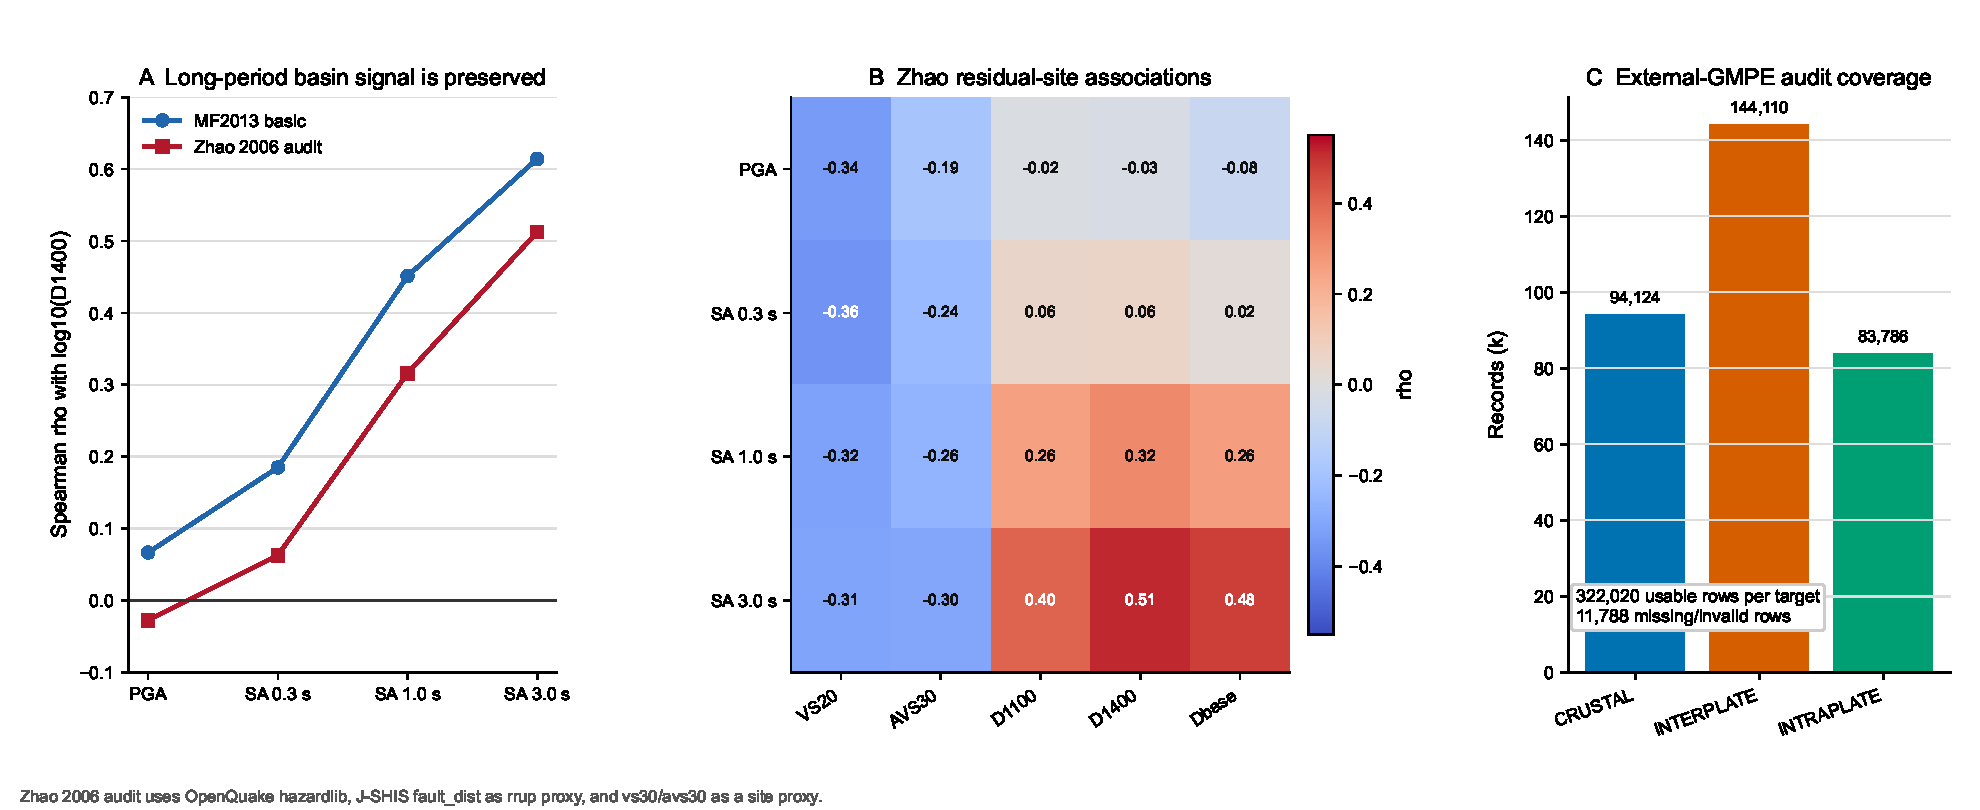
\includegraphics[width=0.90\linewidth]{figures/figure5.pdf}
\caption{External Zhao et al. OpenQuake sensitivity check. PGA shows weak association with D1400; SA(3.0 s) retains a strong basin-depth association. The check uses distance and site proxy inputs.}
\label{fig:s1}
\end{figure}

\begin{figure}[!htbp]
\centering
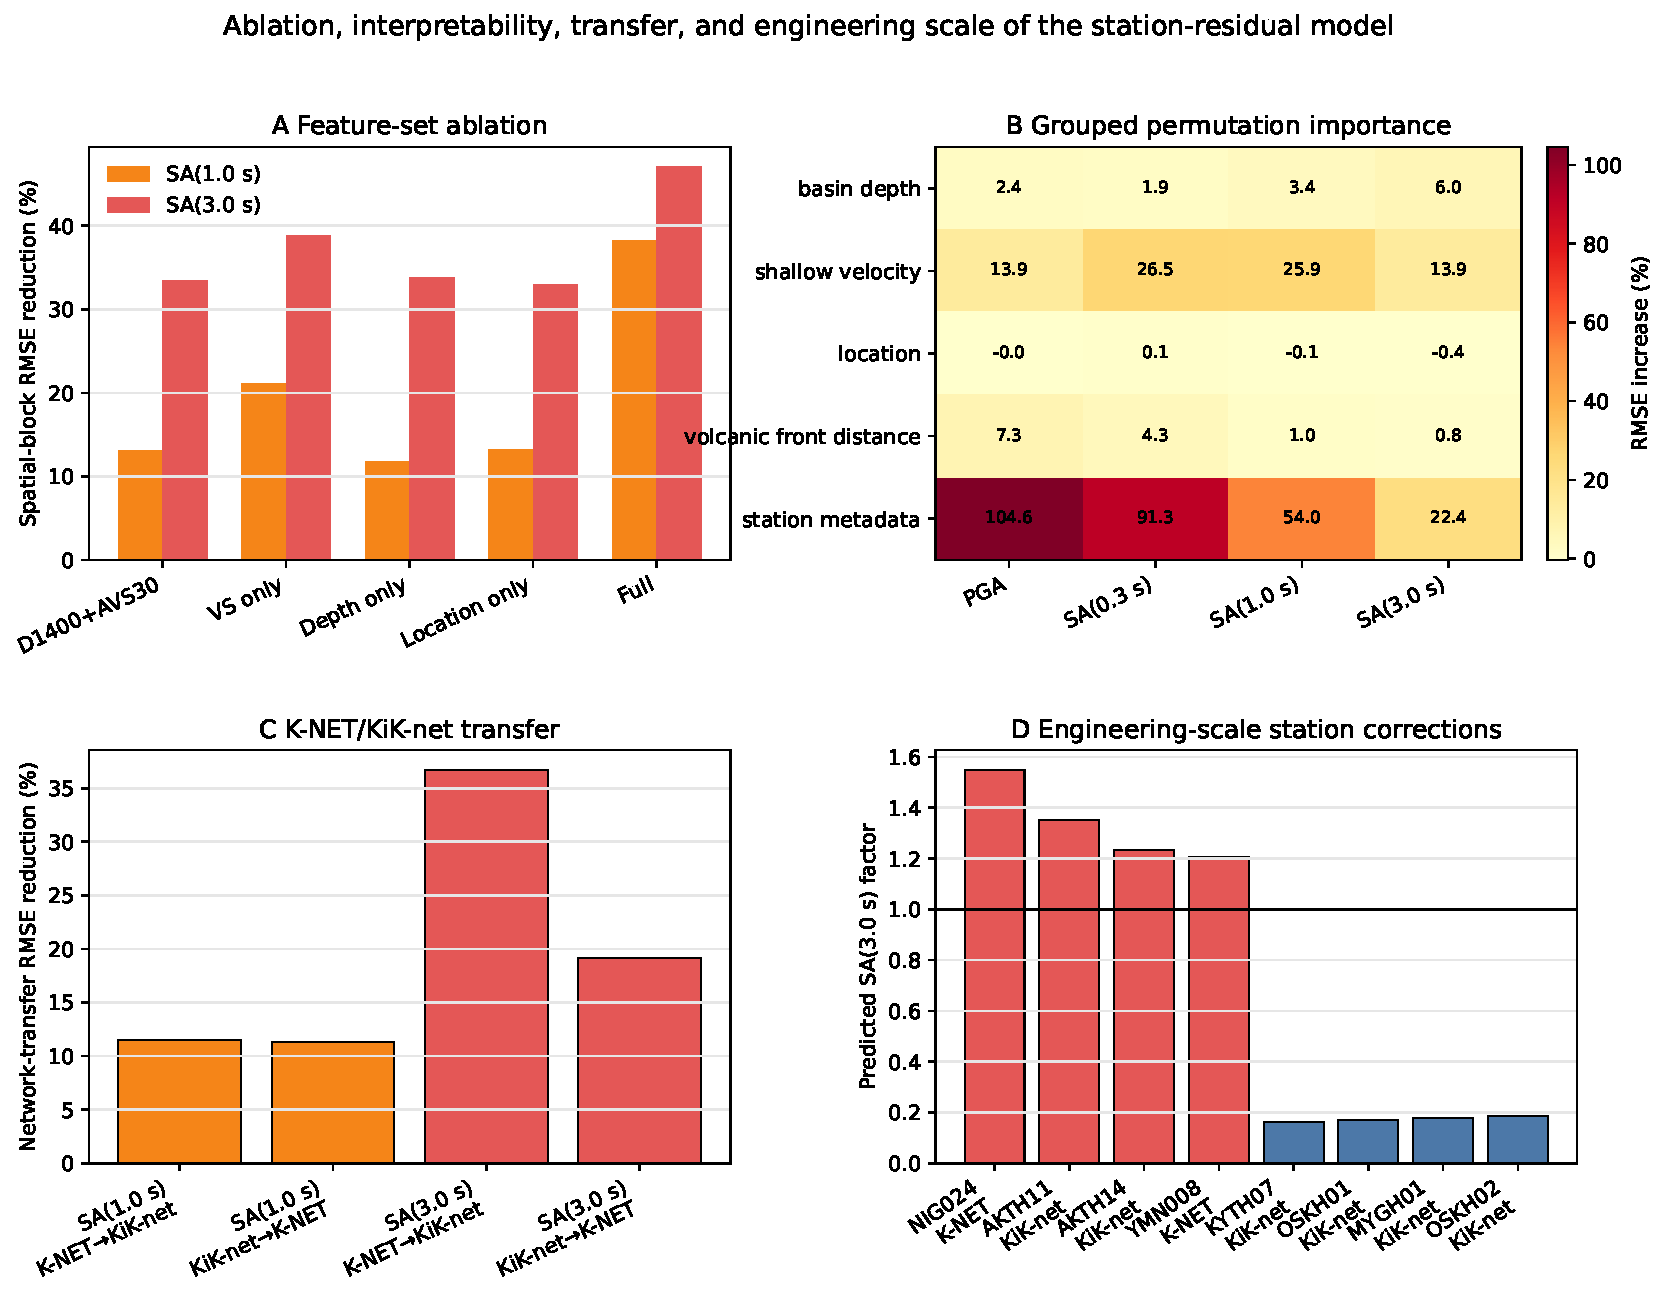
\includegraphics[width=0.96\linewidth]{figures/figure7.pdf}
\caption{Ablation, interpretability, network-transfer validation, and engineering-scale examples for the station-residual model. A: spatial-block feature-set ablation for SA(1.0 s) and SA(3.0 s). B: grouped permutation importance. C: K-NET/KiK-net transfer. D: held-out SA(3.0 s) station correction factors.}
\label{fig:s2}
\end{figure}

\begin{figure}[!htbp]
\centering
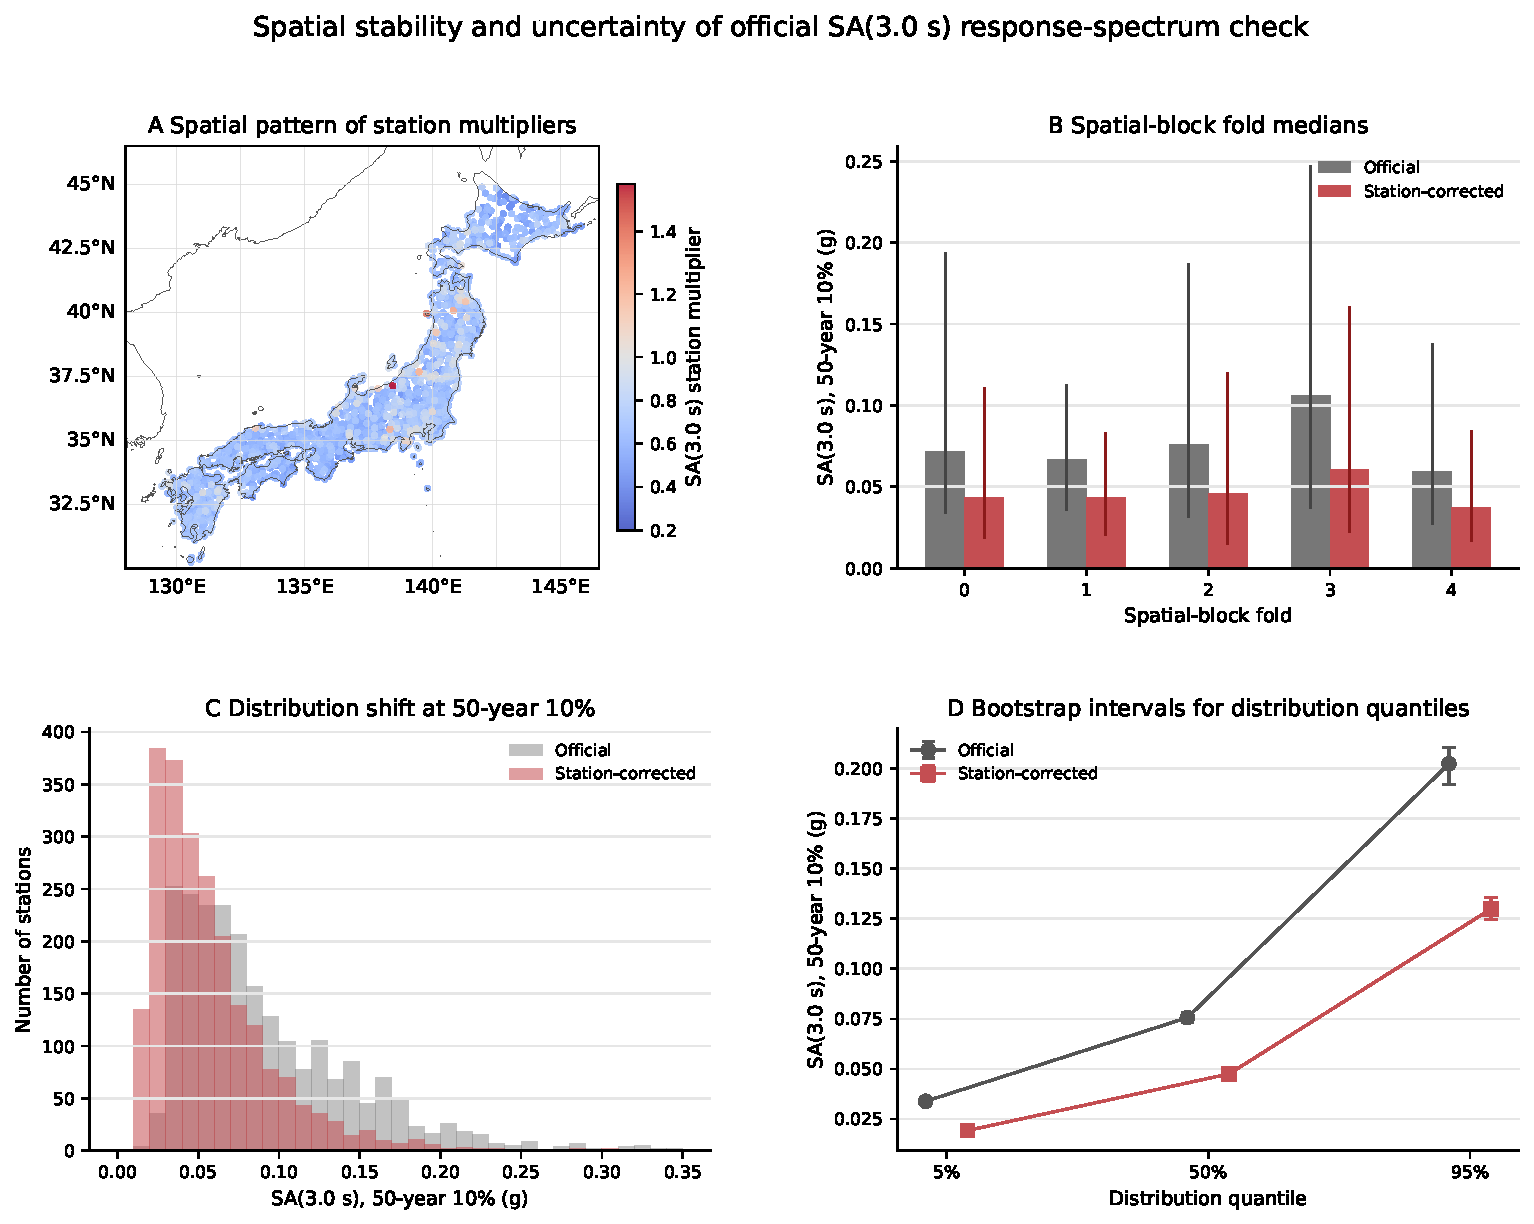
\includegraphics[width=0.96\linewidth]{figures/figure9.pdf}
\caption{Spatial stability and uncertainty of the official SA(3.0 s) response-spectrum check. A: station multiplier map for matched held-out stations. B: spatial-block fold medians, with vertical lines showing 5th--95th percentile ranges. C: distribution shift from official to station-corrected 50-year 10\% SA(3.0 s). D: station-bootstrap 95\% intervals for the 5th, 50th, and 95th percentiles.}
\label{fig:s3}
\end{figure}

\begin{figure}[!htbp]
\centering
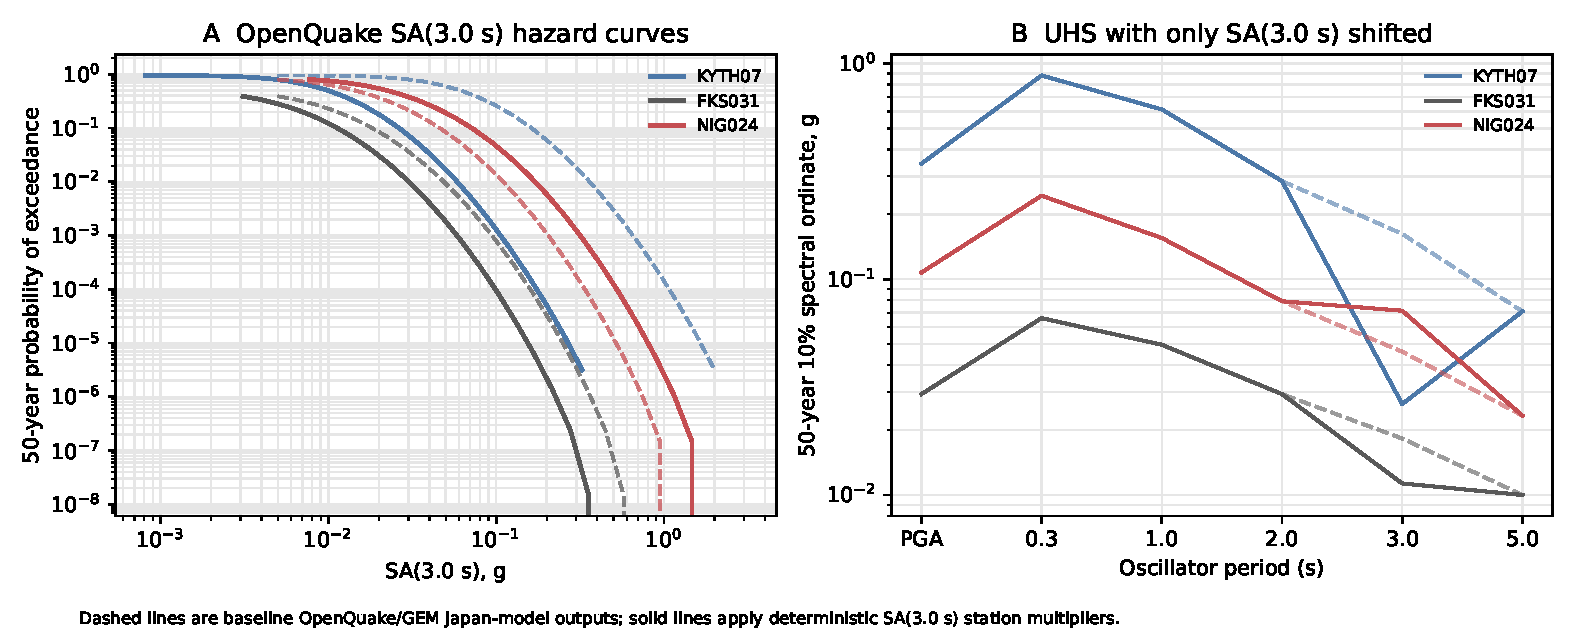
\includegraphics[width=0.96\linewidth]{figures/openquake_jpn_station_psha_sensitivity.pdf}
\caption{Independent OpenQuake/GEM Japan-model PSHA sensitivity check for representative stations. A: mean SA(3.0 s) hazard curves from the OpenQuake baseline calculation, with dashed lines showing baseline curves and solid lines showing deterministic SA(3.0 s) station-multiplier shifts. B: 50-year 10\% uniform-hazard spectra for the same representative stations, with only the SA(3.0 s) ordinate shifted. This supplementary calculation provides an engine-level sensitivity check using packaged OpenQuake Japan mosaic inputs.}
\label{fig:s4}
\end{figure}

\begin{figure}[H]
\centering
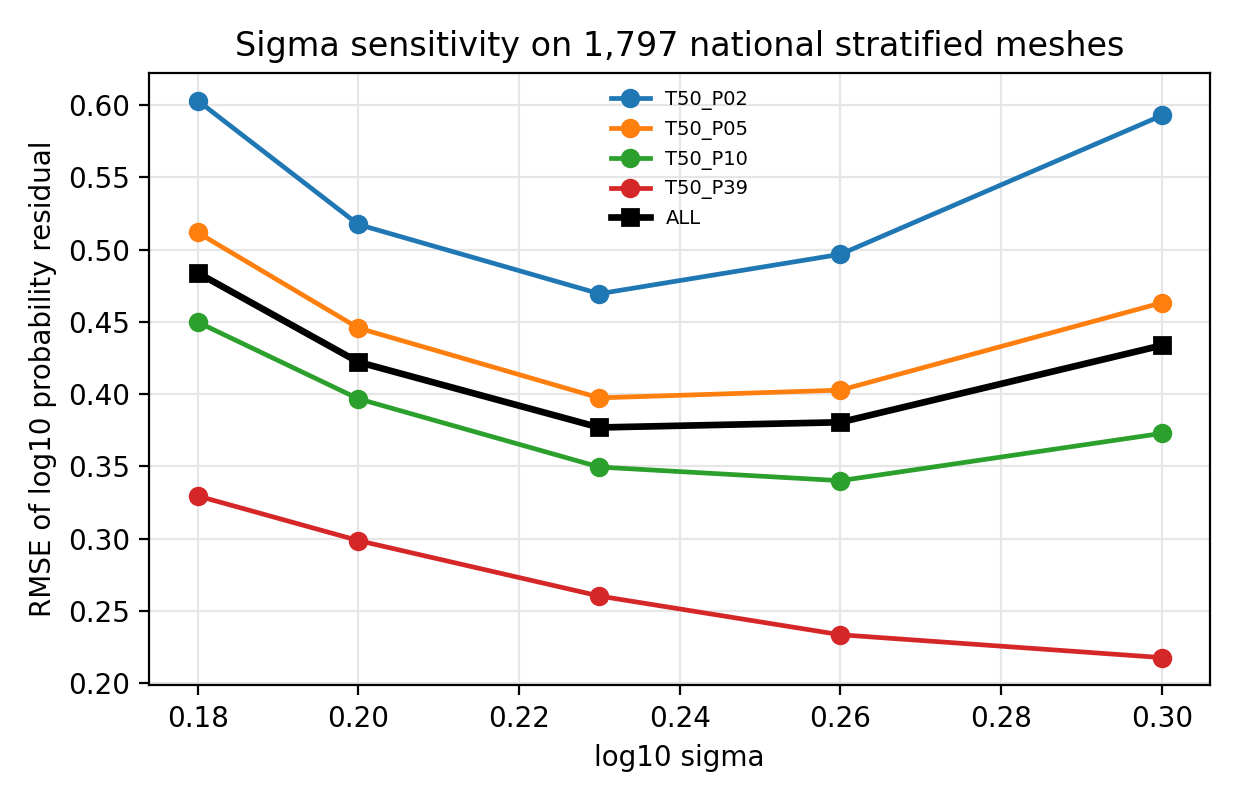
\includegraphics[width=0.86\linewidth]{figures/figure10_sigma_sensitivity.png}
\caption{Five-point sigma sensitivity audit for the public-parameter J-SHIS PBV recomputation. The same 1,797 national stratified meshes are evaluated at log10 sigma values of 0.18, 0.20, 0.23, 0.26, and 0.30. The global RMSE minimum occurs at sigma 0.23; probability-level optima vary across exceedance levels.}
\label{fig:s5}
\end{figure}

\begin{figure}[H]
\centering
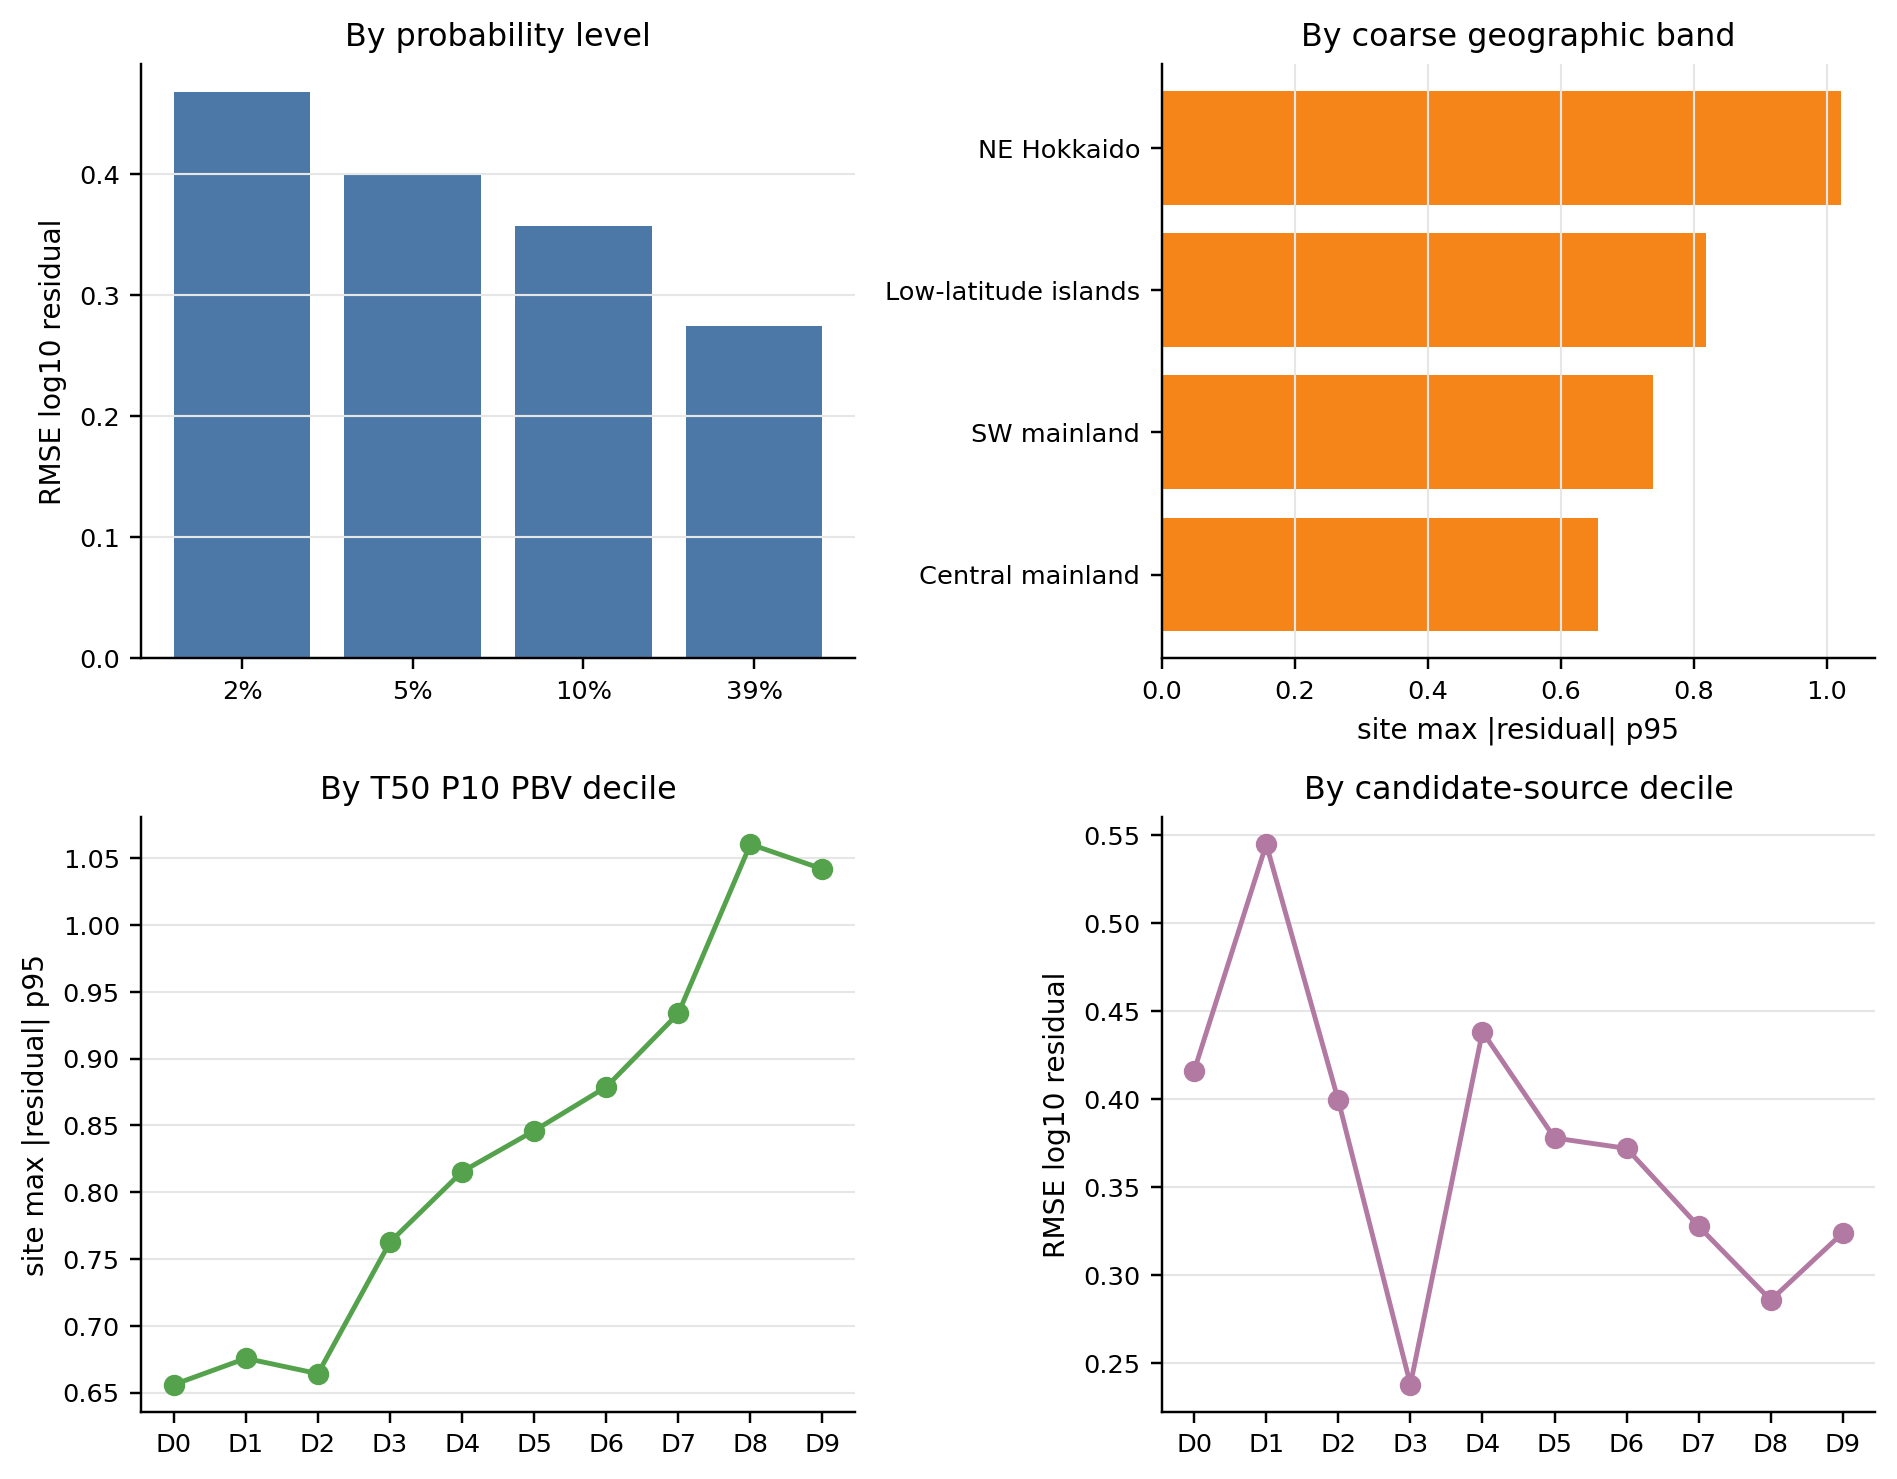
\includegraphics[width=0.96\linewidth]{figures/figure11_residual_root_cause.png}
\caption{Residual-tail diagnostics for the 5,322-mesh public-parameter audit. A: RMSE by official probability level. B: site-level tail amplitude by coarse geographic band. C: site-level tail amplitude by official PBV decile. D: RMSE by candidate-source-count decile. These diagnostics identify structured public-parameter mismatch and confirm valid numerical execution.}
\label{fig:s6}
\end{figure}

\begin{figure}[H]
\centering
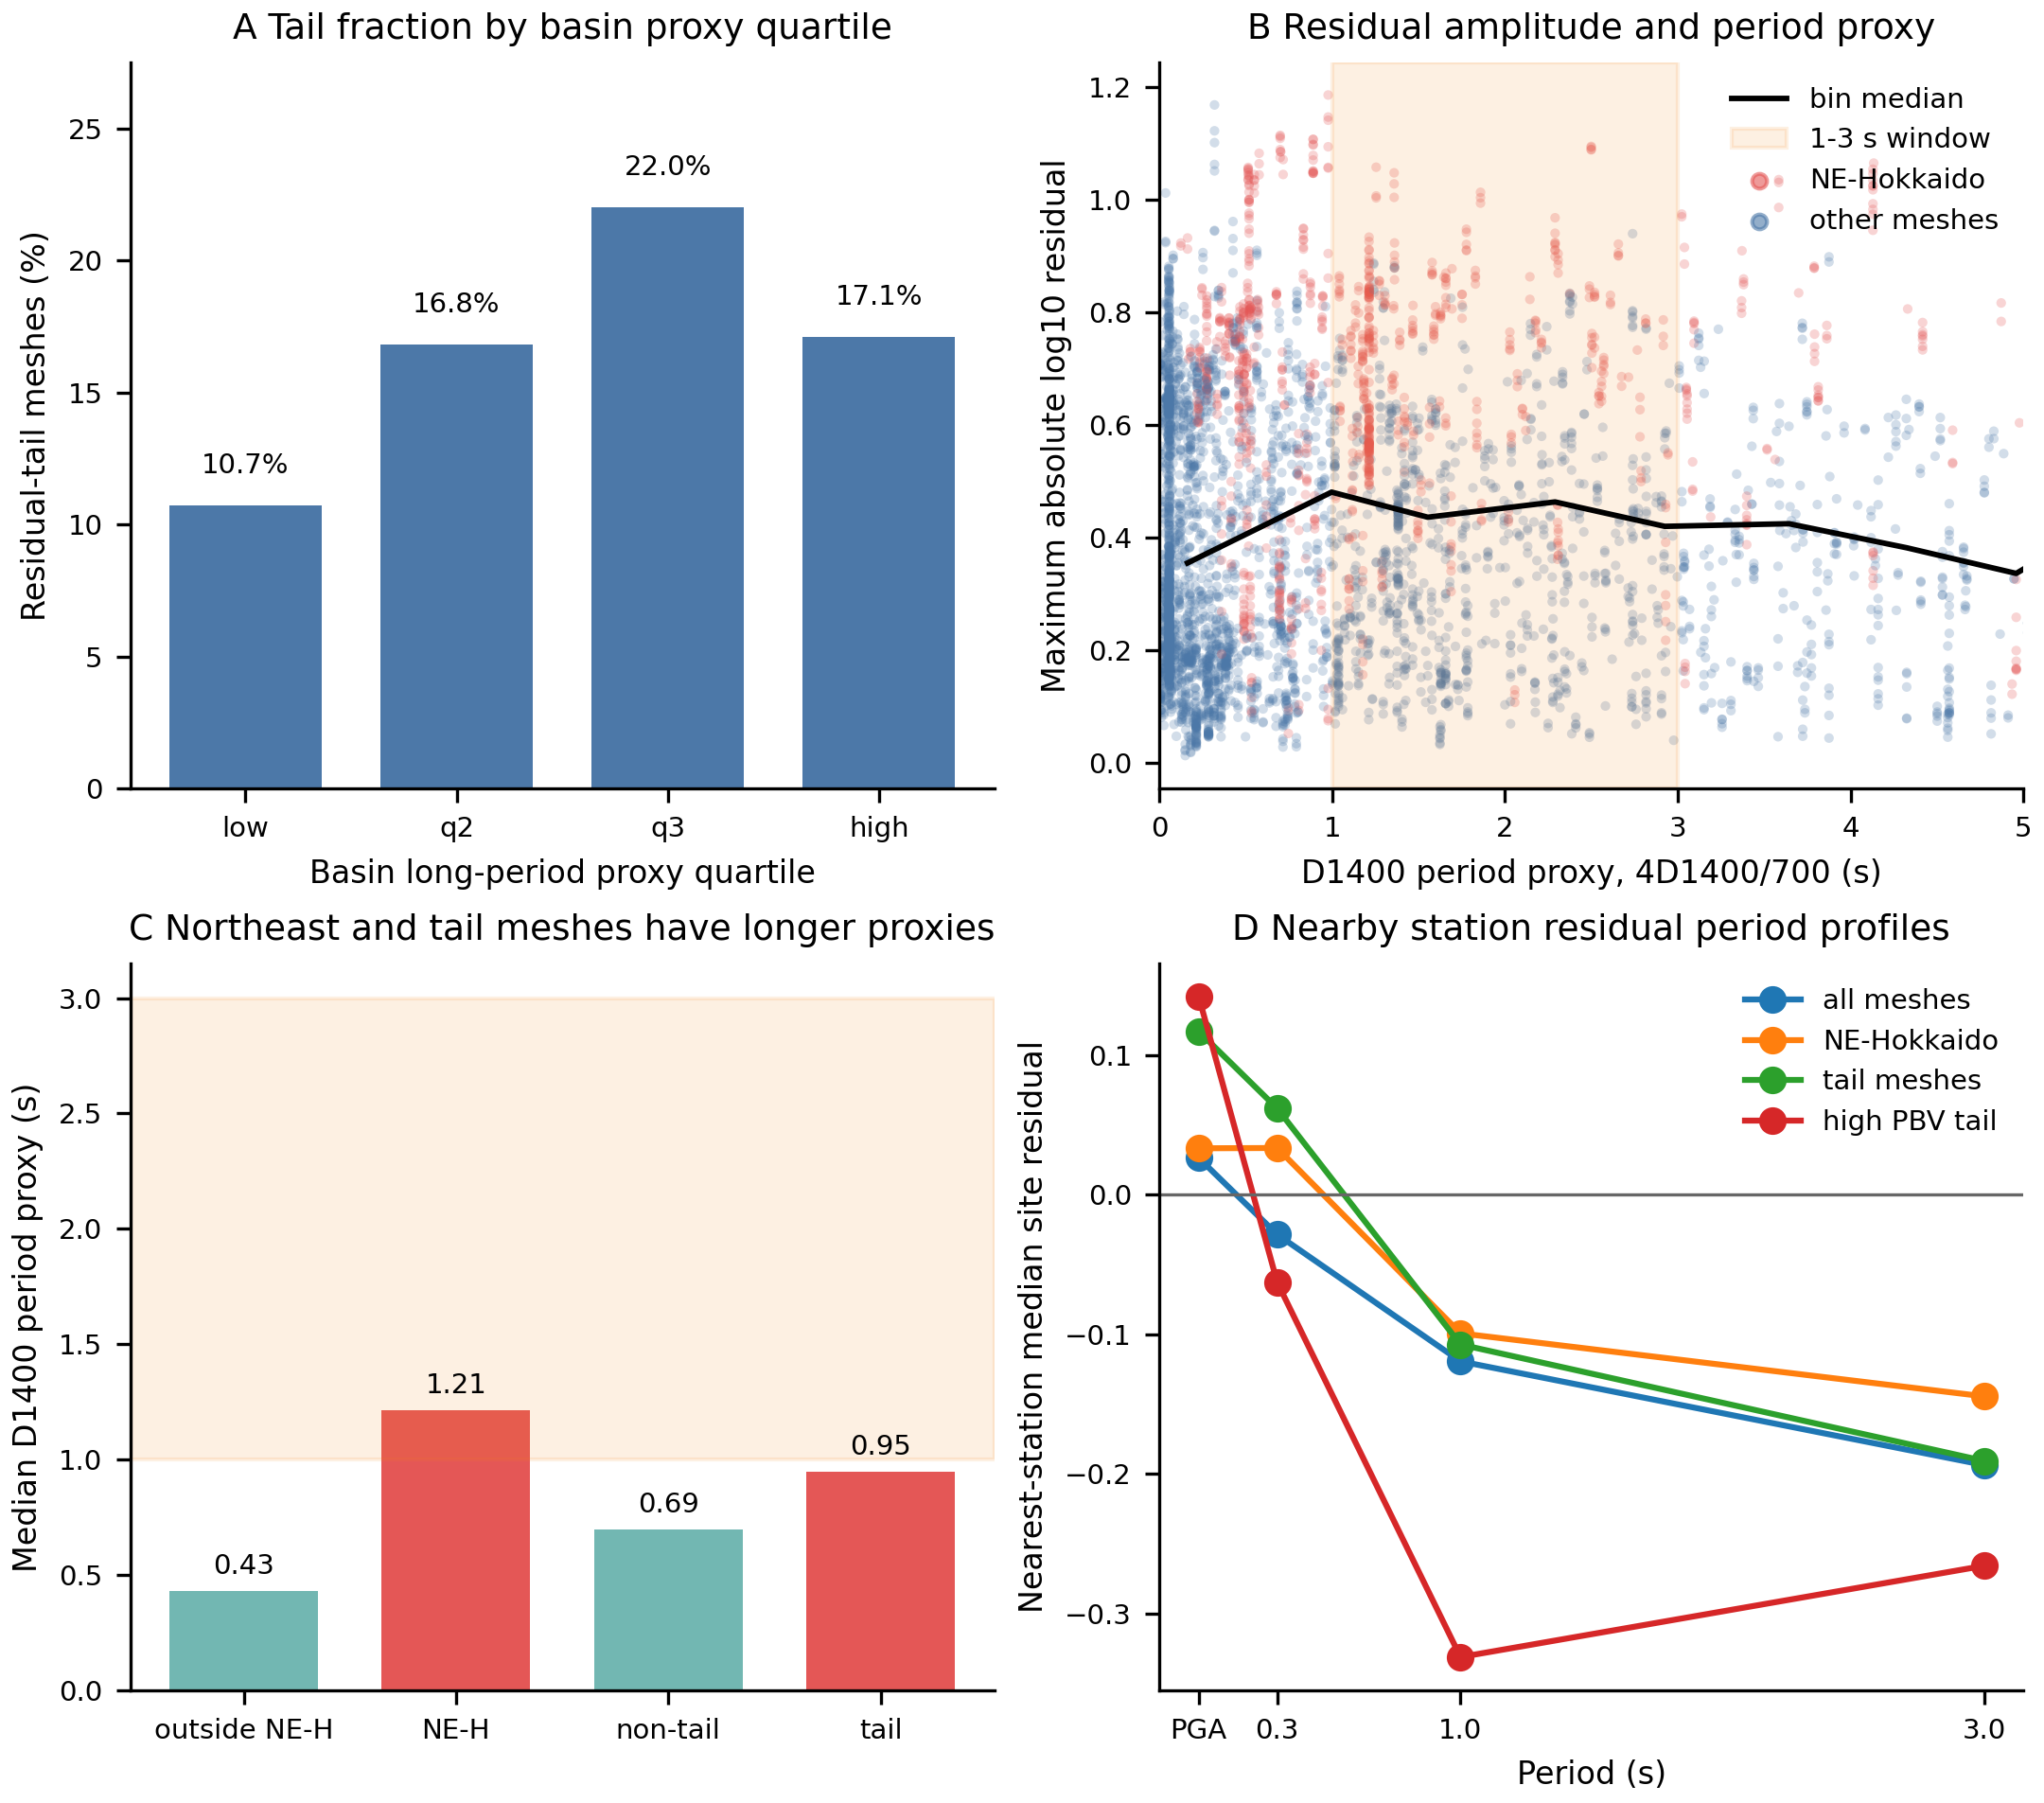
\includegraphics[width=0.99\linewidth]{figures/figure12_basin_period_proxy.png}
\caption{Basin-period proxy audit for the 10,467-mesh public-parameter residual-tail structure. A: residual-tail fraction by basin long-period proxy quartile. B: maximum absolute log10 residual against the D1400-derived period proxy 4D1400/700, with the 1--3 s window shaded. C: median D1400-derived period proxy for northeast-Hokkaido, outside-northeast-Hokkaido, residual-tail, and non-tail meshes. D: nearby-station MF2013 site-corrected residual period profiles for all meshes, northeast-Hokkaido meshes, residual-tail meshes, and high-PBV tail meshes.}
\label{fig:s7}
\end{figure}

\begin{figure}[H]
\centering
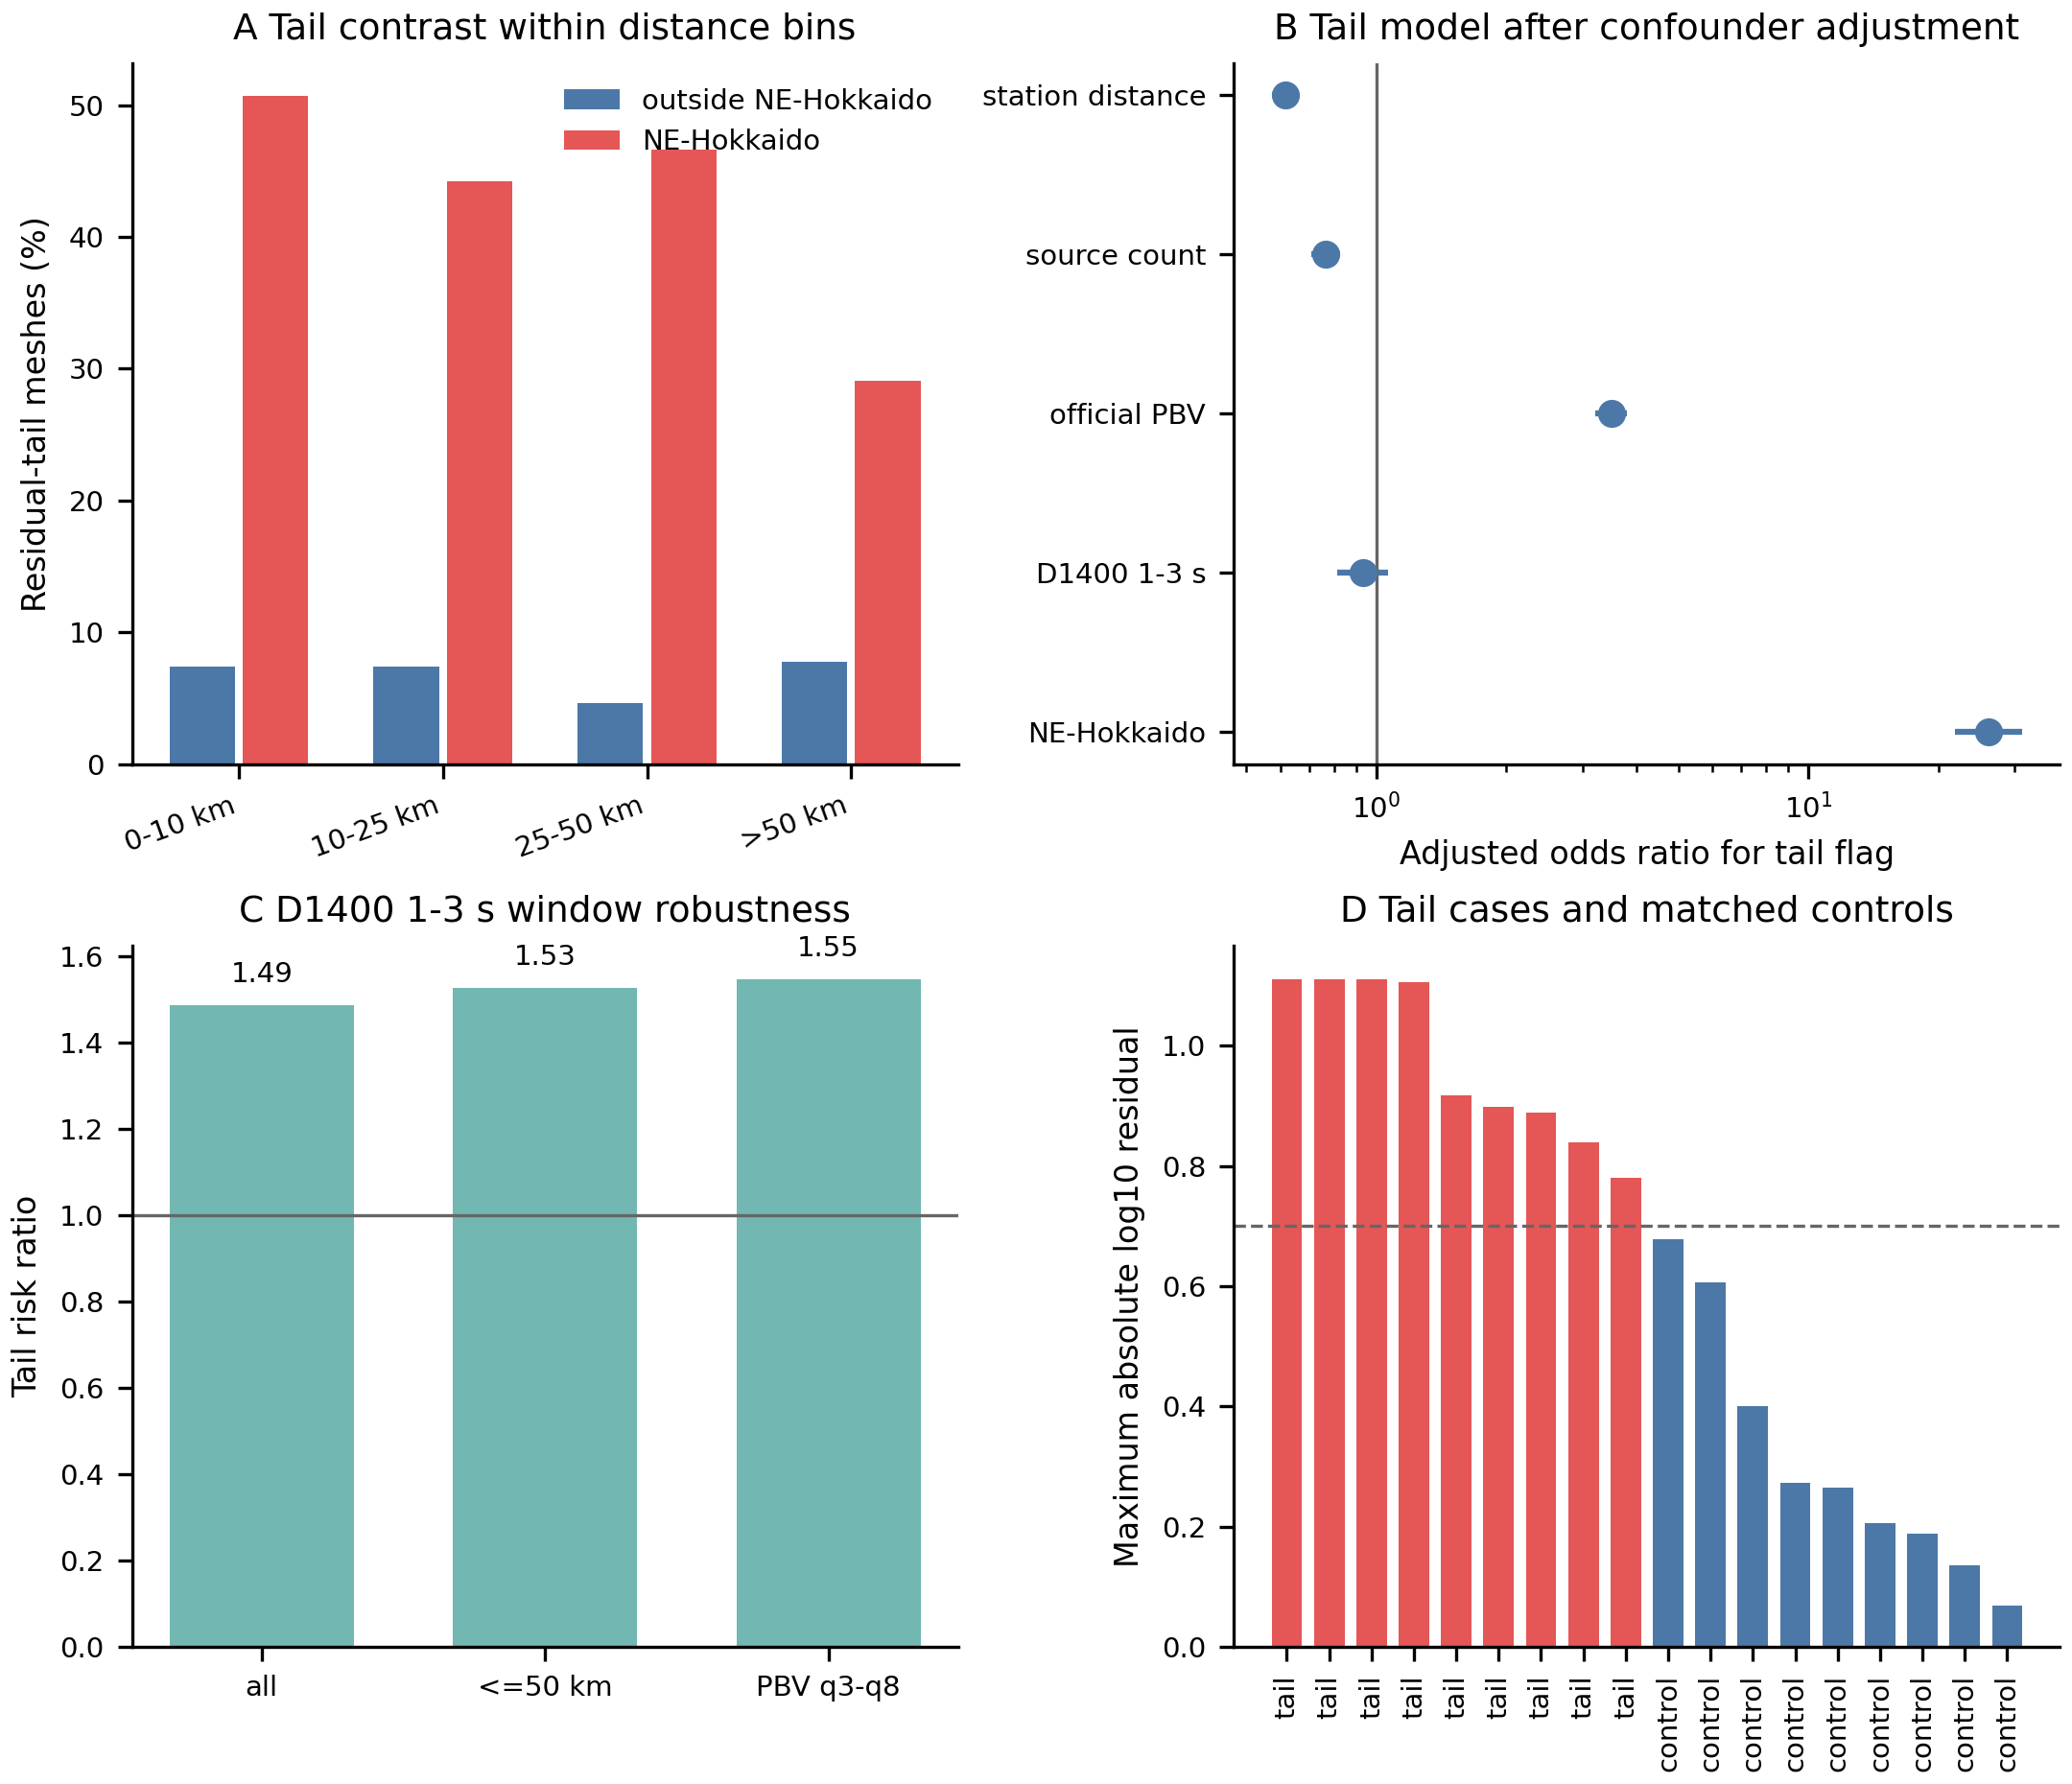
\includegraphics[width=0.99\linewidth]{figures/figure13_tail_robustness_cases.png}
\caption{Tail-robustness and matched-case audit for the 10,467-mesh public-parameter residual-tail structure. A: residual-tail fraction in northeast-Hokkaido and outside-northeast-Hokkaido meshes within station-distance bins. B: adjusted odds ratios from a logistic tail model with official PBV, candidate-source count, station distance, station residual contrast, northeast-Hokkaido membership, and the D1400-derived 1--3 s proxy window. C: tail-risk ratios for the D1400-derived 1--3 s proxy window across all meshes, the nearest-station $\leq$50 km subset, and middle official-PBV deciles q3--q8. D: maximum absolute log10 residuals for matched tail and non-tail mesh profiles.}
\label{fig:s8}
\end{figure}

\begin{figure}[H]
\centering
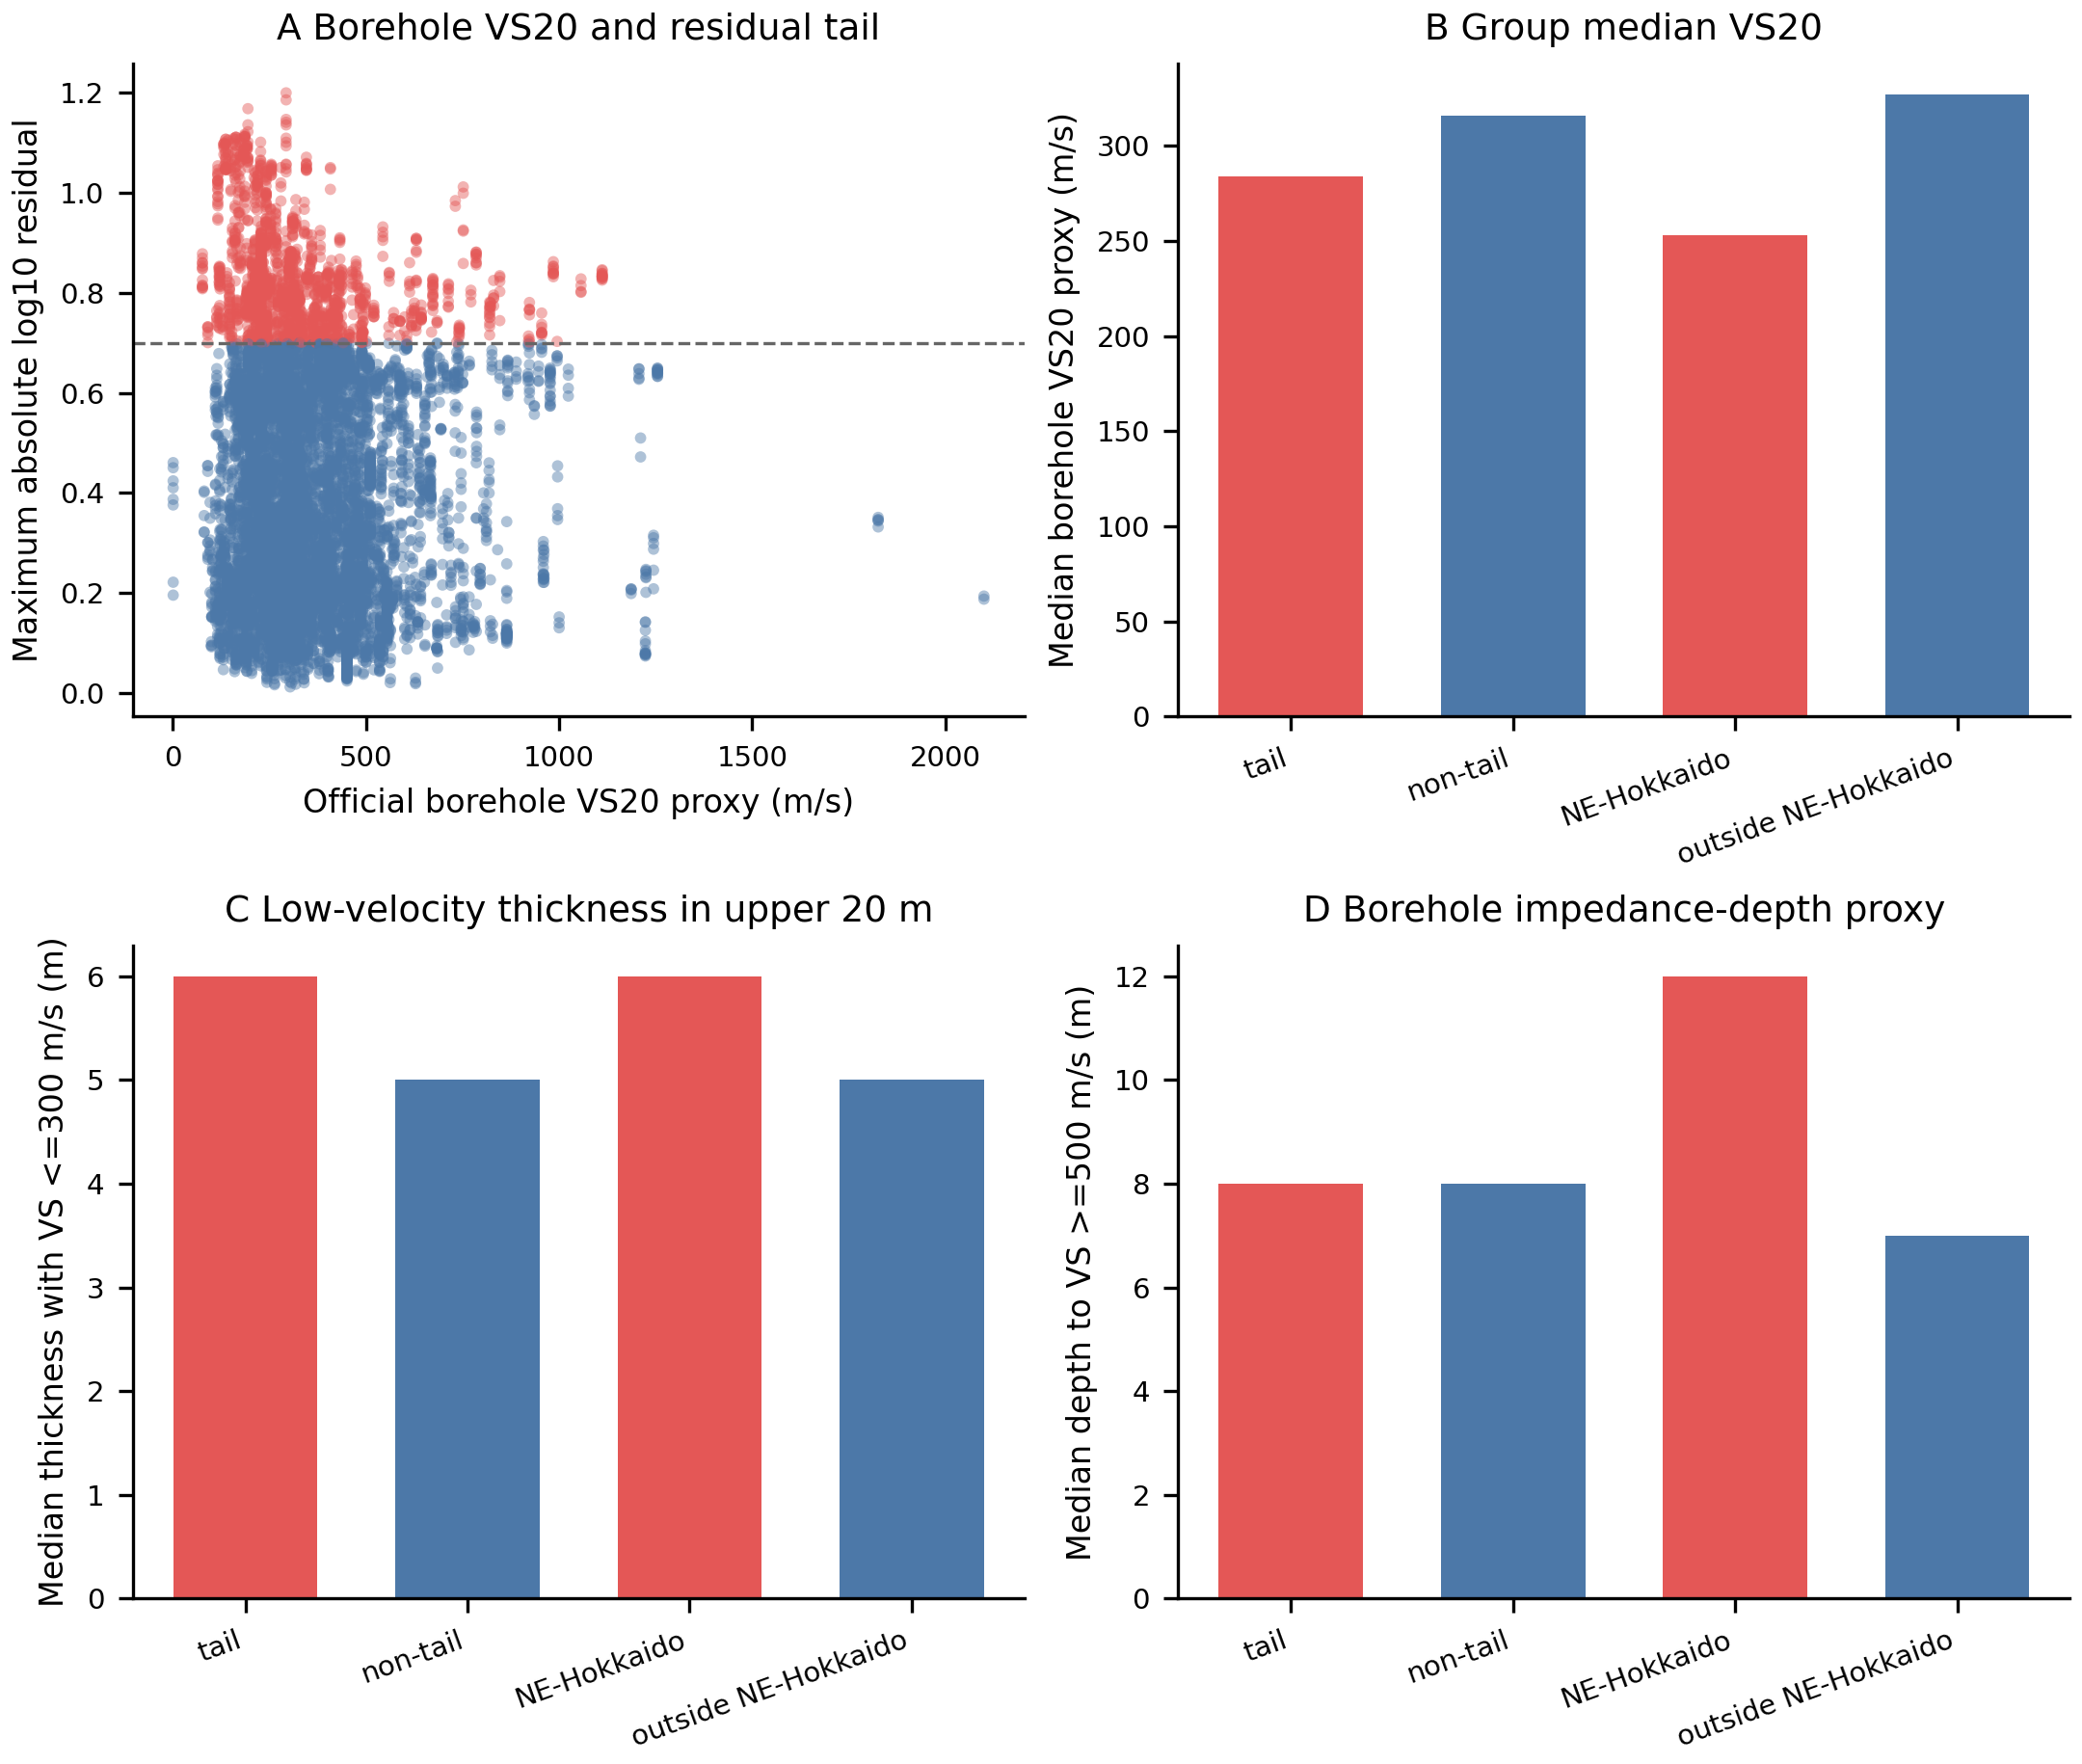
\includegraphics[width=0.96\linewidth]{figures/figure14_nearest_station_borehole_audit.png}
\caption{Nearest-station official borehole-profile audit for the 10,467-mesh public-parameter residual-tail structure. A: maximum absolute log10 residual against the public NIED borehole VS20 proxy for the nearest K-NET/KiK-net station, with residual-tail meshes highlighted. B: median borehole VS20 proxy for tail, non-tail, northeast-Hokkaido, and outside-northeast-Hokkaido groups. C: median upper-20 m thickness with VS $\leq$300 m/s. D: median depth to VS $\geq$500 m/s. The audit provides a nearest-station profile check for proxy-level interpretation.}
\label{fig:s9}
\end{figure}

\begin{figure}[H]
\centering
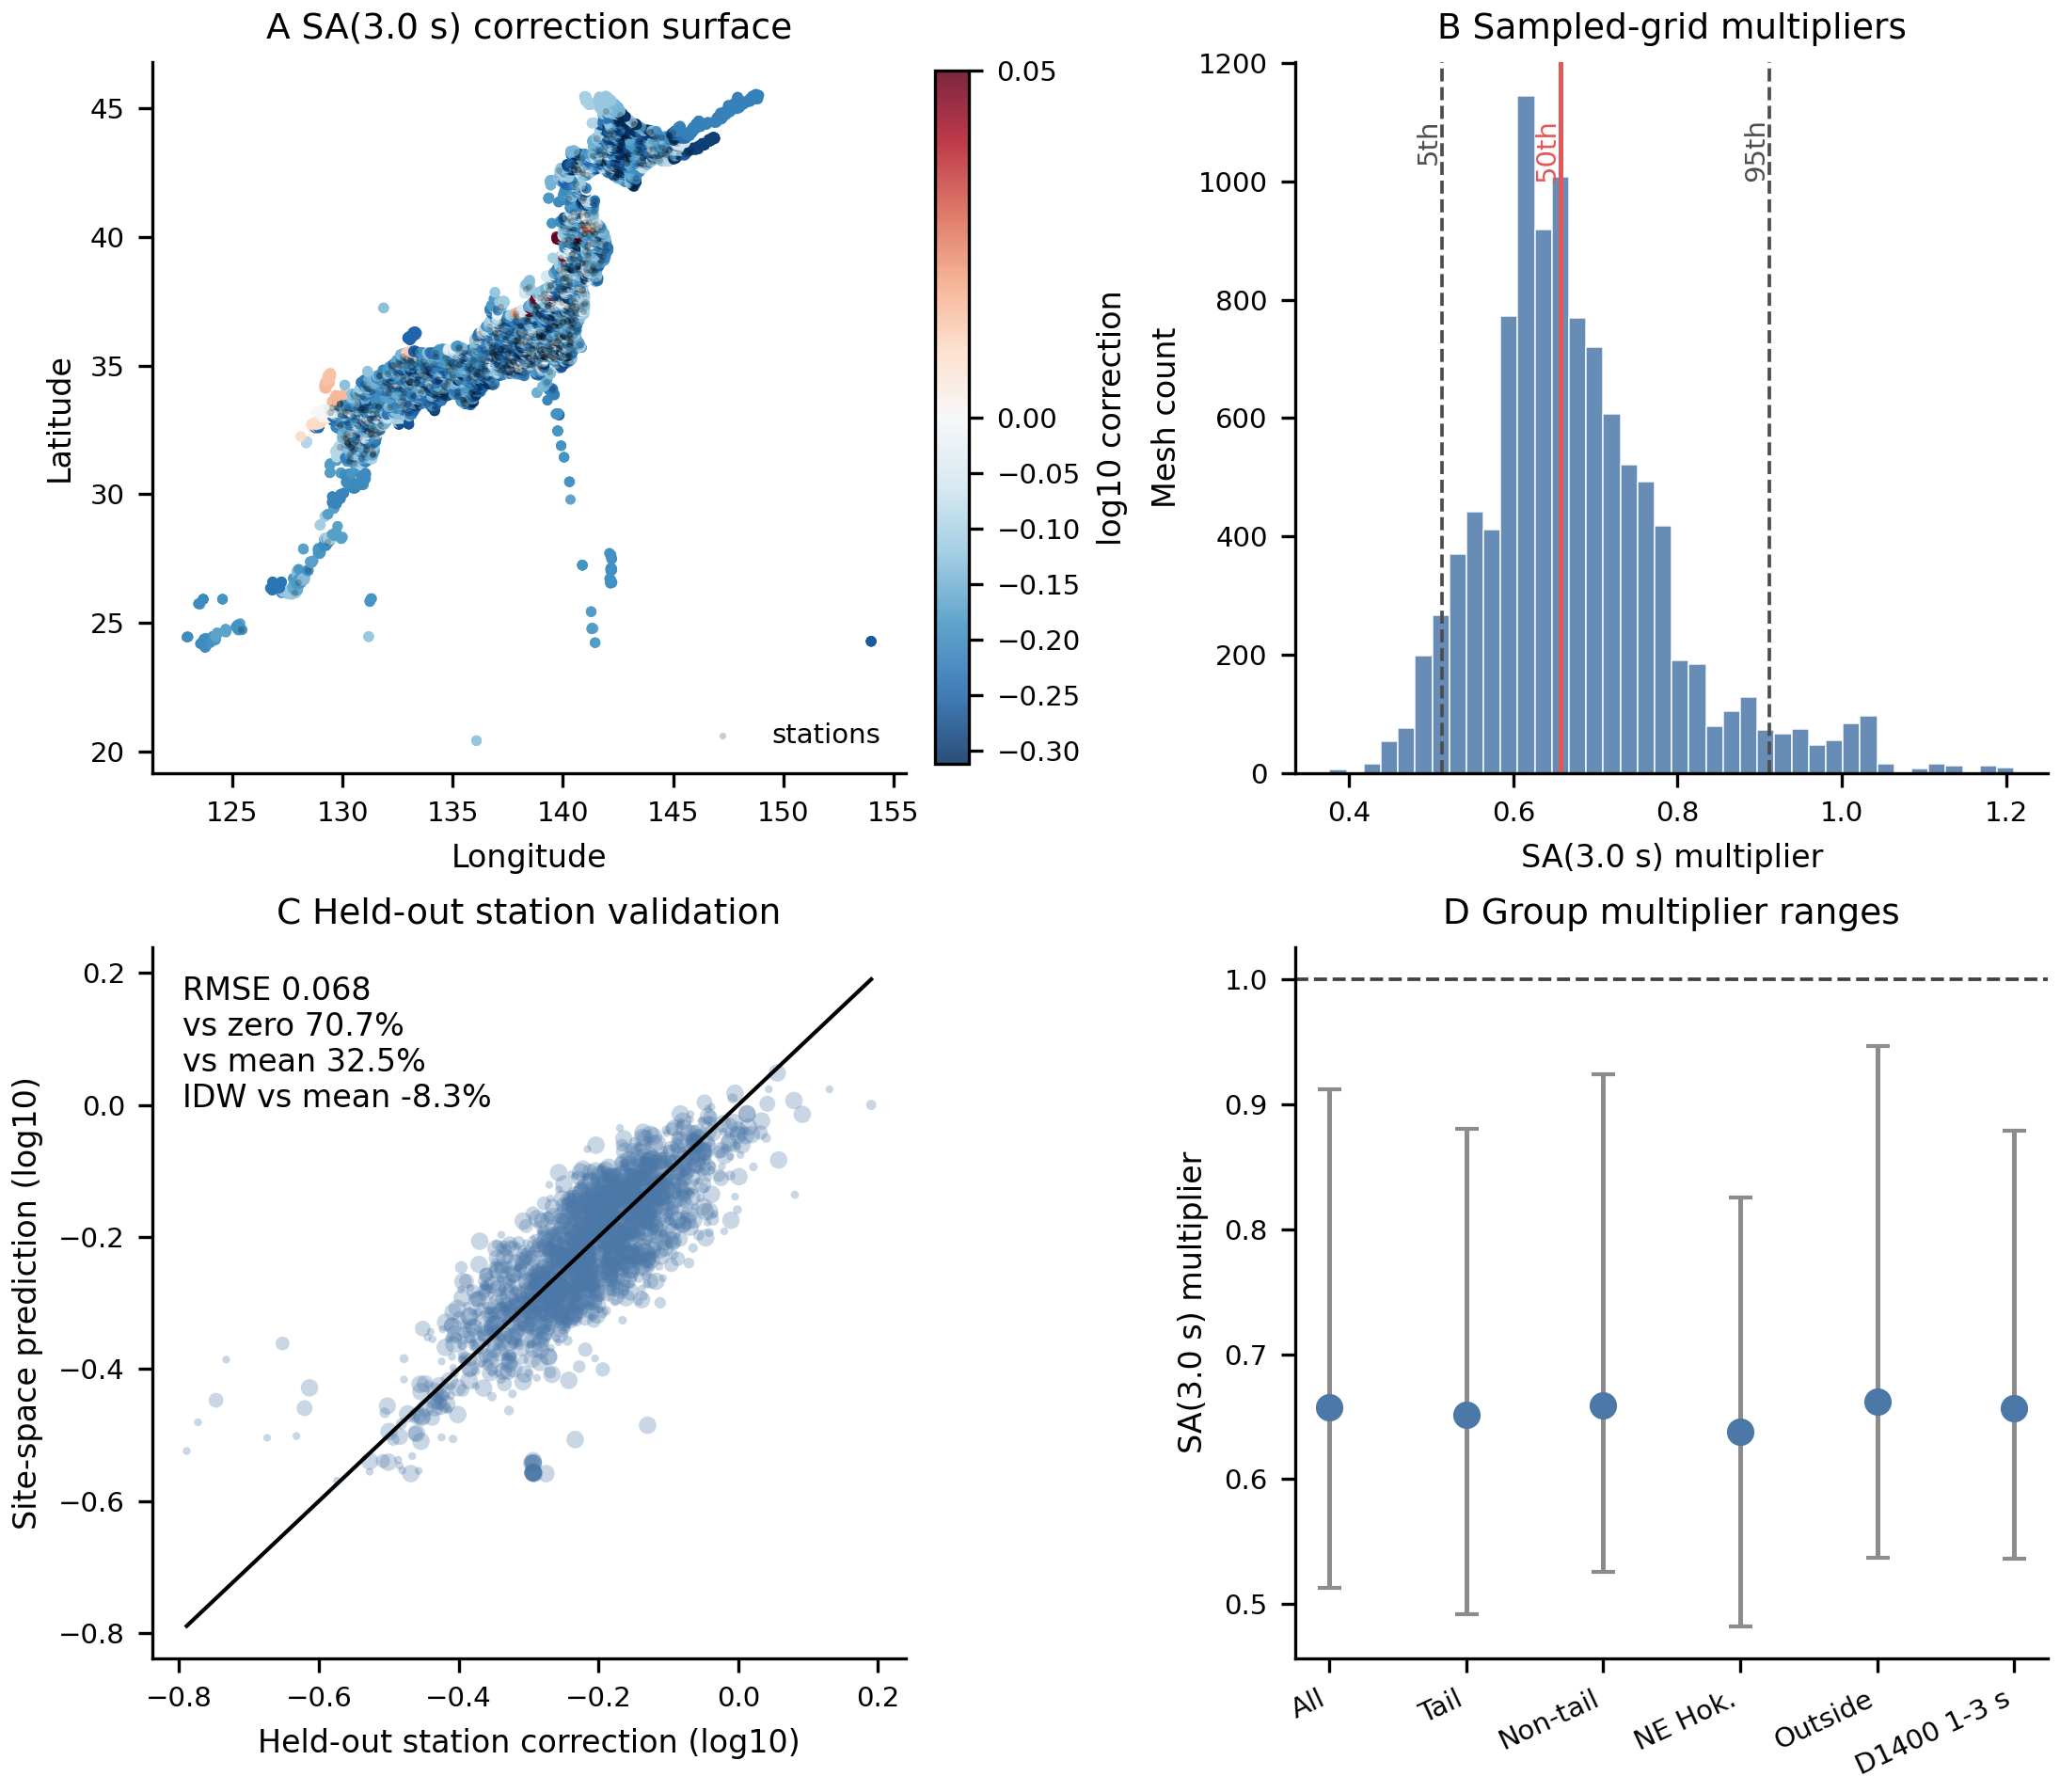
\includegraphics[width=0.96\linewidth]{figures/figure15_sa3_continuous_surface.png}
\caption{Sampled-grid SA(3.0 s) continuous correction-surface audit. A: site-and-location gradient-boosted correction surface on the 10,467-mesh public-parameter audit grid, with station locations shown for reference. B: sampled-grid multiplier distribution. C: spatial-block held-out station validation for the site-and-location surface. D: group median multipliers with 5th--95th percentile ranges. The sampled-grid values use nearest-station public site proxies and test the station-to-grid continuity step.}
\label{fig:s10}
\end{figure}

\begin{figure}[H]
\centering
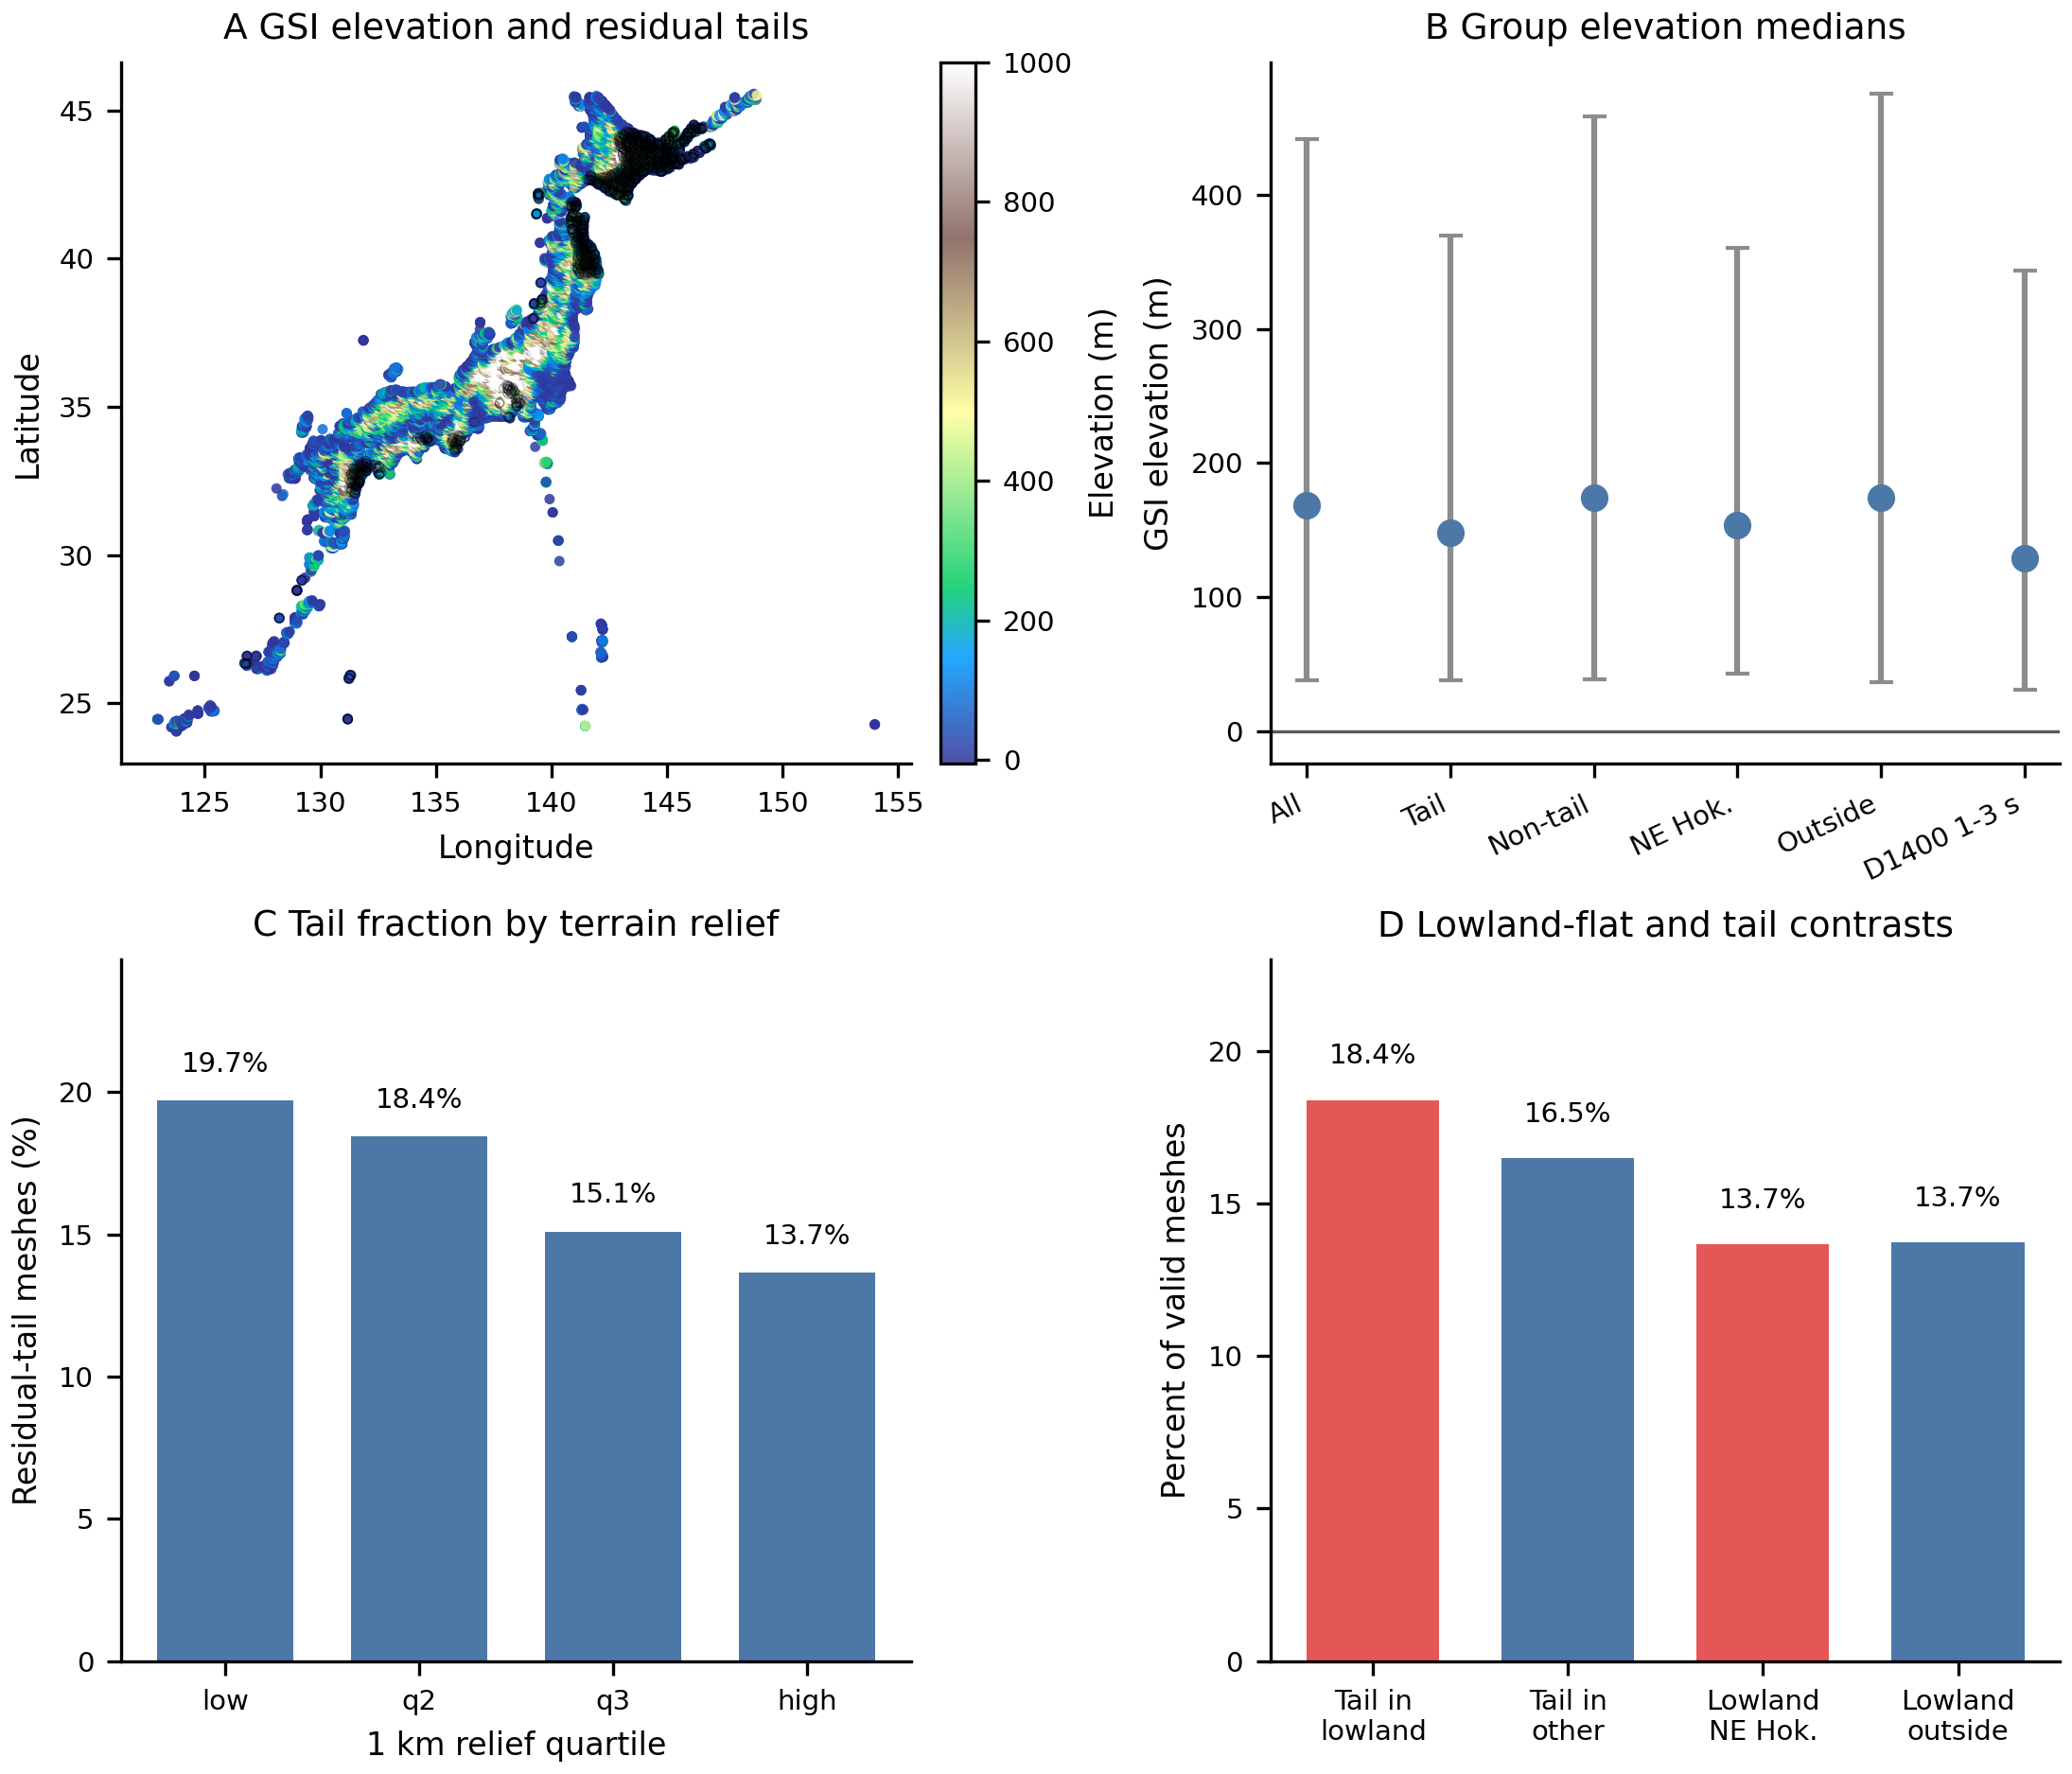
\includegraphics[width=0.96\linewidth]{figures/figure16_gsi_terrain_geomorphic_audit.png}
\caption{Independent GSI terrain geomorphic proxy audit for the 10,467-mesh public-parameter residual-tail structure. A: GSI elevation sampled from public DEM PNG tiles, with residual-tail meshes outlined. B: group elevation medians with interquartile ranges. C: residual-tail fraction by 1 km relief quartile. D: lowland-flat terrain and residual-tail contrasts. The audit tests external surface-geomorphic consistency; shear-wave velocity and three-dimensional basin geometry require separate data.}
\label{fig:s11}
\end{figure}

\begin{figure}[H]
\centering
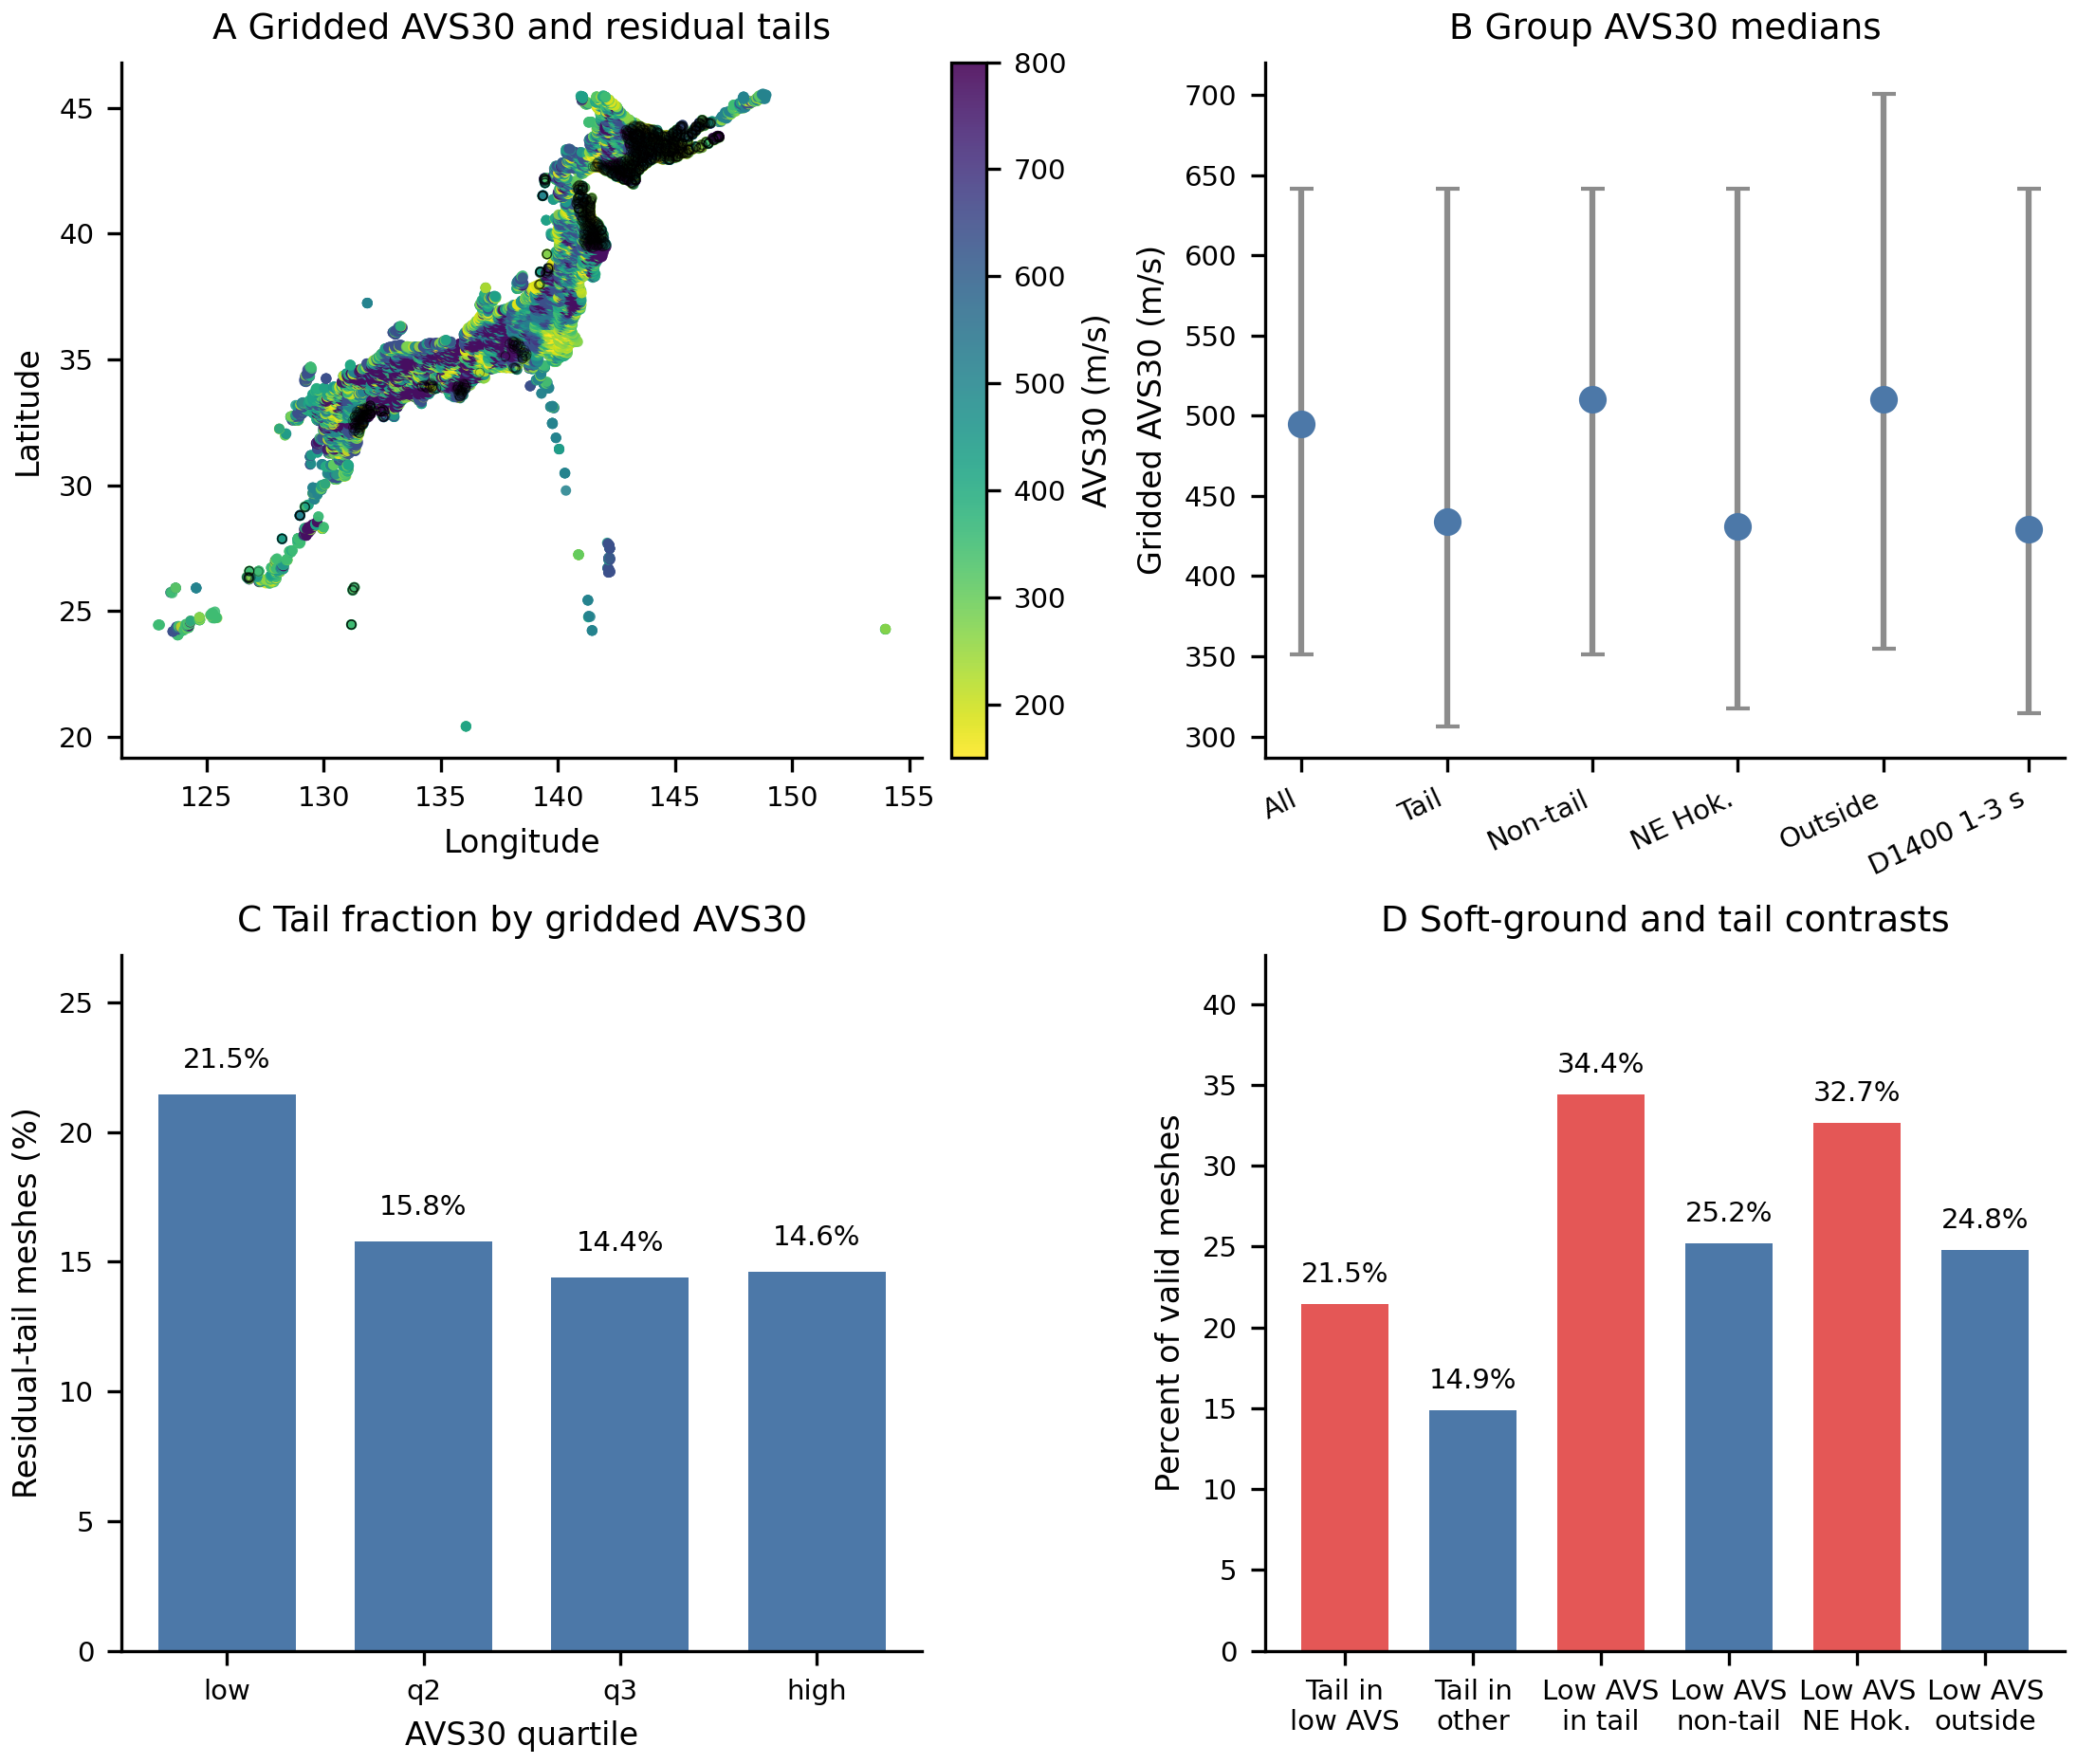
\includegraphics[width=0.96\linewidth]{figures/figure17_zamp_vs400_site_amplification_audit.png}
\caption{J-SHIS VS400 site-amplification layer audit for the 10,467-mesh public-parameter residual-tail structure. A: gridded AVS30 from the public 250 m surface-ground layer, with residual-tail meshes outlined. B: group AVS30 medians with interquartile ranges. C: residual-tail fraction by gridded AVS30 quartile. D: soft-ground and residual-tail contrasts. The audit supplies gridded shallow-velocity and surface-amplification context for the residual-tail interpretation.}
\label{fig:s12}
\end{figure}

\begin{figure}[H]
\centering
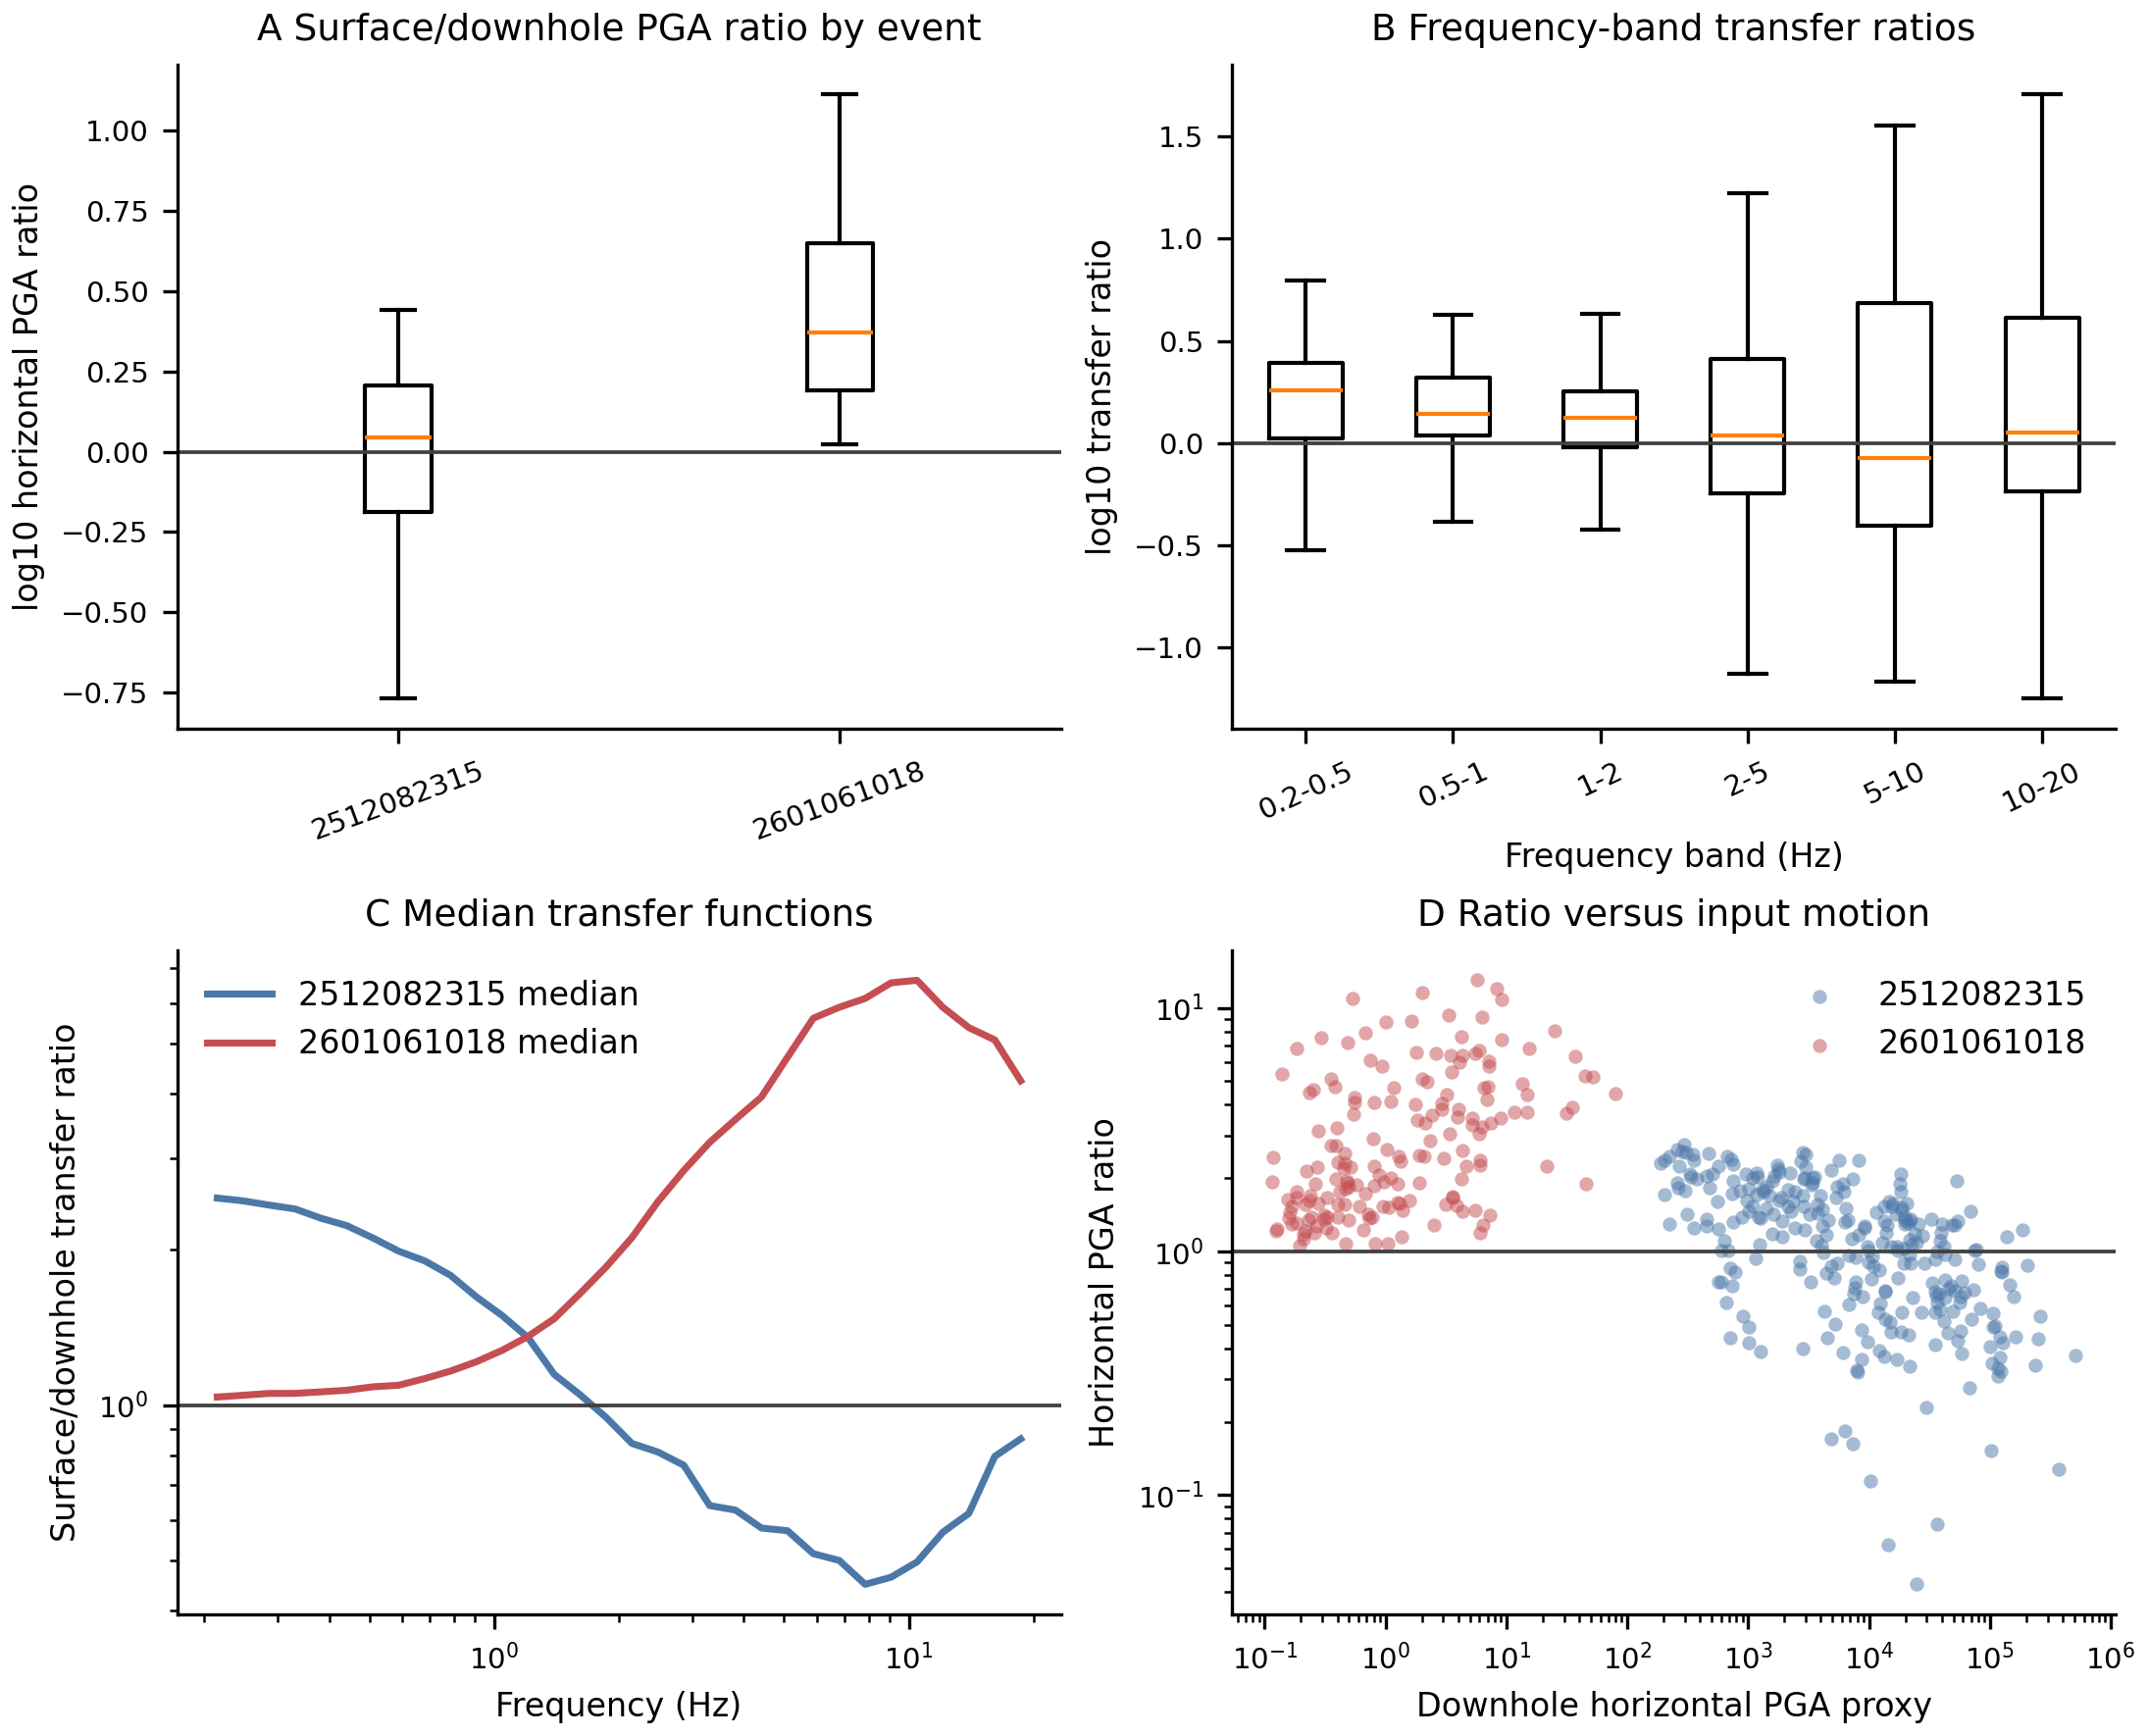
\includegraphics[width=0.96\linewidth]{figures/figure16_kiknet_multievent_transfer_function.png}
\caption{Multi-event KiK-net surface/downhole transfer-function audit. A: horizontal PGA ratio by event. B: frequency-band transfer-ratio distributions for 460 event-station pairs. C: event-wise median transfer functions. D: horizontal PGA ratio against downhole input-motion proxy. The audit combines 288 converted miniSEED surface/downhole pairs and 172 NIED ASCII pairs converted with header scale factors.}
\label{fig:s13}
\end{figure}

\begin{figure}[H]
\centering
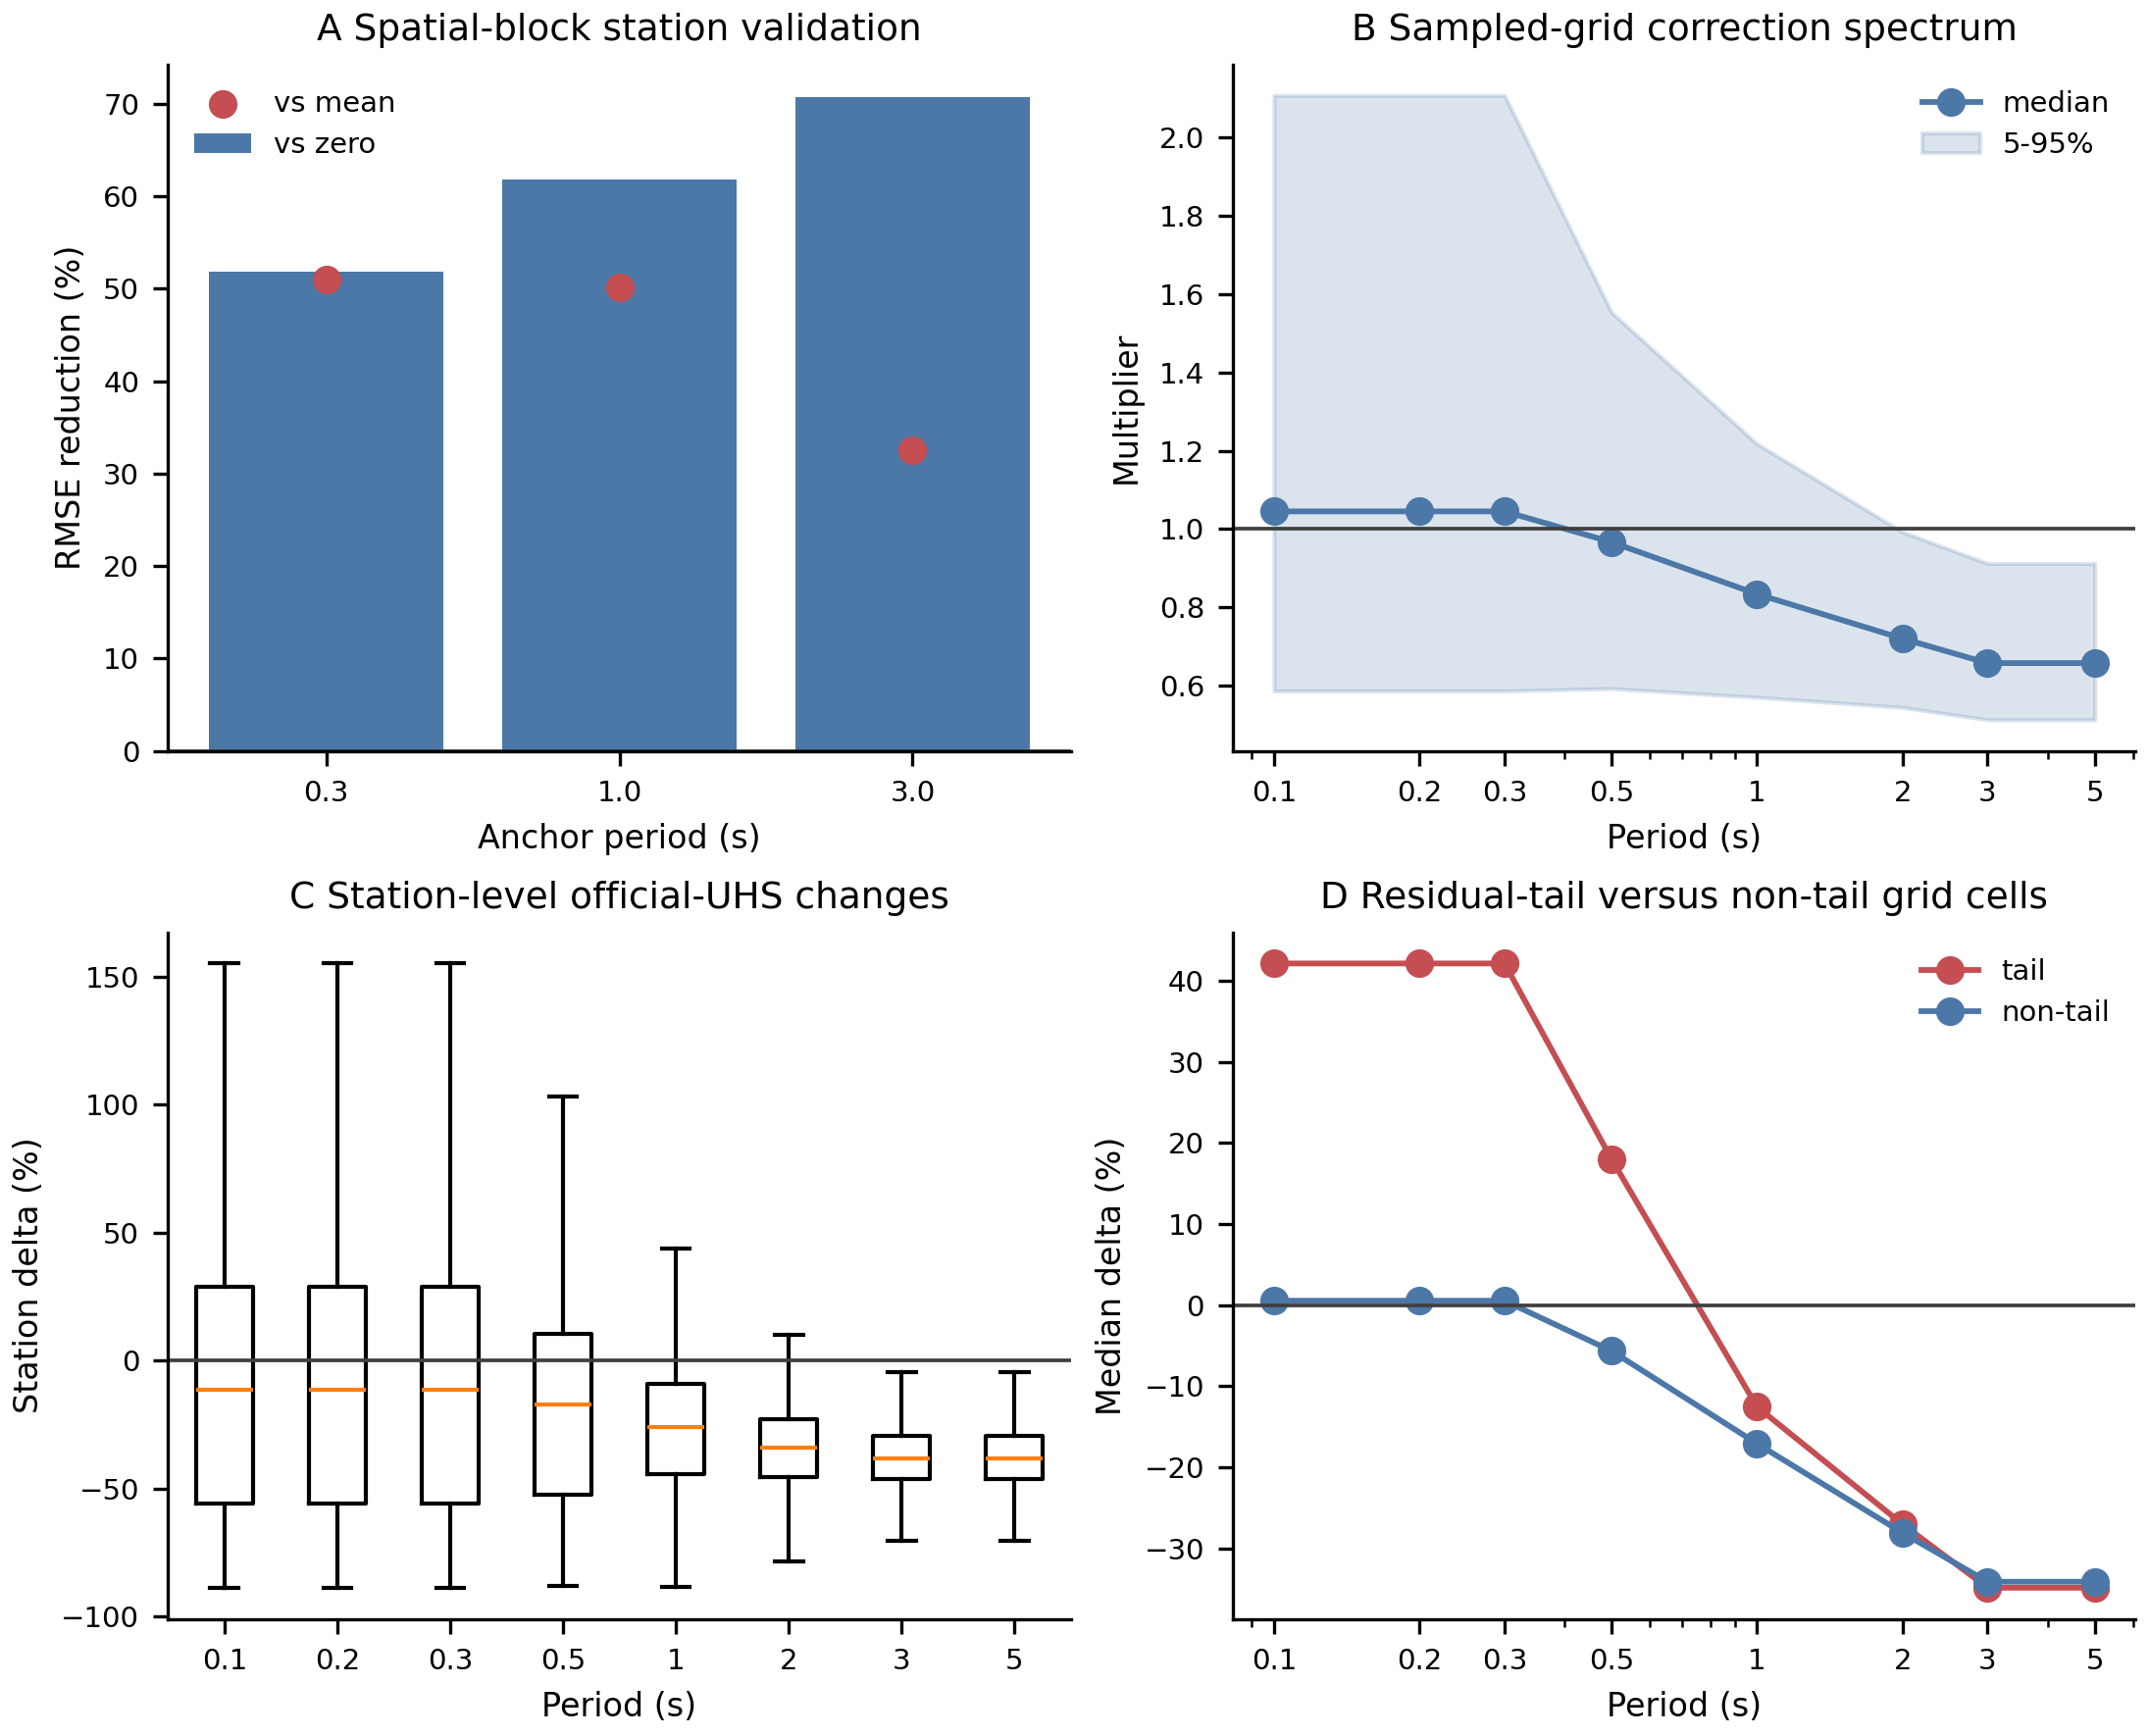
\includegraphics[width=0.96\linewidth]{figures/figure17_multiperiod_nonergodic_psha.png}
\caption{All-period official-response-spectrum non-ergodic propagation audit. A: spatial-block held-out station validation for SA(0.3 s), SA(1.0 s), and SA(3.0 s) correction surfaces. B: sampled-grid 50-year 10\% multiplier spectrum on 10,467 meshes. C: matched-station official-UHS percent changes. D: residual-tail and non-tail sampled-grid median changes by period. The calculation propagates station terms through official J-SHIS response-spectrum map ordinates and keeps the official source model and uncertainty settings fixed.}
\label{fig:s14}
\end{figure}

\begin{figure}[H]
\centering
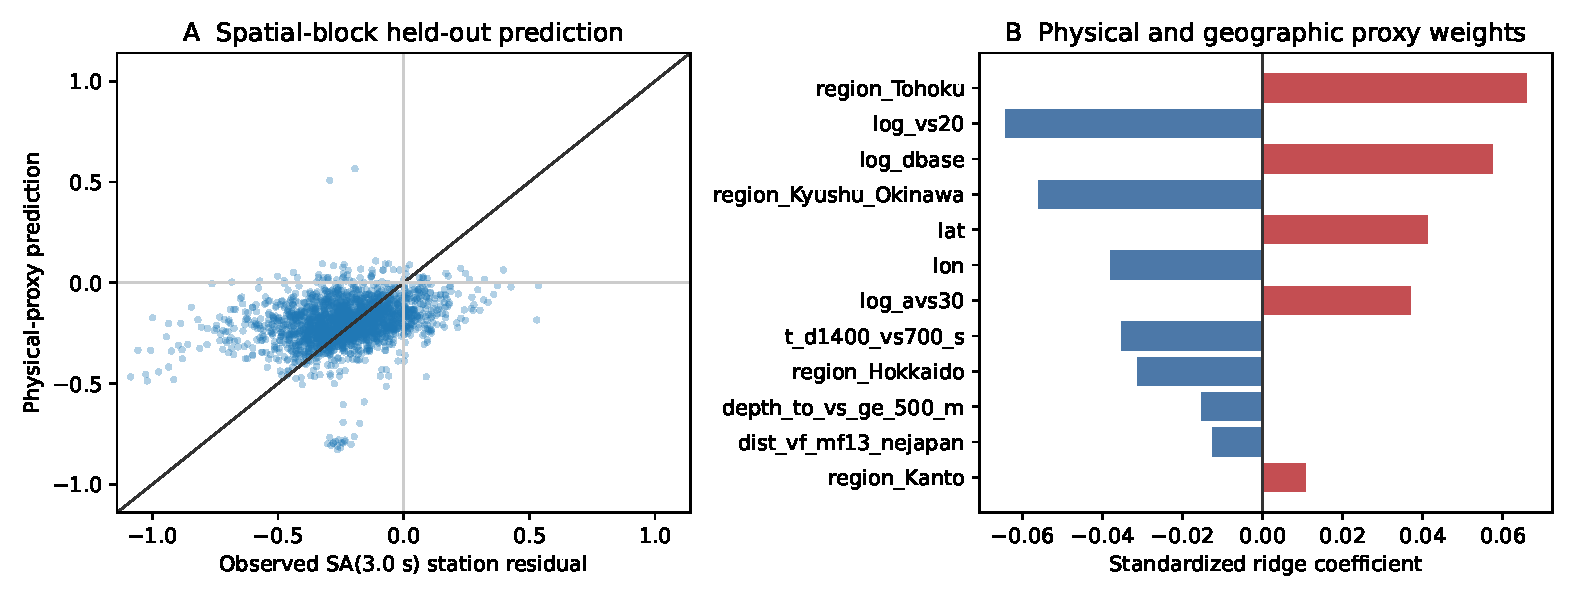
\includegraphics[width=0.96\linewidth]{figures/figure18_sa3_physical_proxy_model.pdf}
\caption{Interpretable SA(3.0 s) site-variable model. A: spatial-block held-out observed and predicted MF2013 site-corrected station residuals. B: largest standardized ridge-regression coefficients. Predictors include basin-depth proxies, shallow-velocity proxies, public borehole-profile proxies, volcanic-front distances, elevation, sensor depth, coordinates, and broad Japanese region.}
\label{fig:s15}
\end{figure}

\section*{Supplementary Tables and Audit Files}

The accompanying \path{supplement/} directory contains machine-readable CSV and Markdown audit files for the additional validation checks.

\begingroup
\scriptsize
\sloppy
\setlength{\emergencystretch}{2em}
\begin{itemize}
\setlength{\itemsep}{0.05em}
\setlength{\parsep}{0pt}
\setlength{\parskip}{0pt}
\item Supplementary Table S1: \path{jshis_station_matching_missingness_audit.csv}. This file documents 333,808 public flatfile records, 2,581 record station identifiers, 2,607 site-schema rows, complete record-to-site matching, and site-variable availability.
\item Supplementary Table S2: \path{jshis_station_region_leaveout_summary.csv} and \path{jshis_station_region_leaveout_fold_metrics.csv}. These files report seven-region geographic leave-out validation for the station-residual model.
\item Supplementary Table S3: \path{jshis_station_variable_substitution_summary.csv}, \path{jshis_station_site_variable_collinearity_pairs.csv}, and \path{jshis_station_site_variable_vif.csv}. These files report official-variable substitutions and collinearity checks for D1400, AVS30, VS20, and Dbase.
\item Supplementary Table S4: \path{jshis_official_hazard_response_summary.csv}. This file reports official and SA(3.0 s)-corrected response-spectrum ordinates at 50-year 2\%, 5\%, 10\%, and 39\% exceedance probabilities.
\item Supplementary Table S5: \path{jshis_positive_sa3_station_correction_summary.csv} and \path{jshis_positive_sa3_station_correction_audit.csv}. These files identify the 24 matched stations with positive SA(3.0 s) correction factors and list their site-level values.
\item Supplementary Table S6: \path{jshis_official_data_provenance_2026-06-14.csv}, \path{cee_code_data_release_manifest_2026-06-14.md}, and \path{cee_release_metadata_zenodo_draft.json}. These files provide data-source provenance, redistribution boundaries, and DOI-deposition metadata for release preparation.
\item Supplementary Table S7: \path{jshis_existing_sensitivity_inventory.csv} and \path{jshis_existing_influence_and_external_model_sensitivity.md}. These files inventory the existing event-exclusion, station-exclusion, magnitude-bin, distance-bin, and Zhao et al. external-model sensitivity outputs.
\item Supplementary Table S8: \path{openquake_jpn_station_psha_summary.csv}, \path{openquake_jpn_station_psha_uhs.csv}, \path{openquake_jpn_station_psha_hazard_curves.csv}, and \path{openquake_jpn_station_psha_sensitivity.md}. These files report the independent OpenQuake/GEM Japan-model PSHA sensitivity calculation for five representative stations.
\item Supplementary Table S9: \path{jshis_public_psha_national_stratified5322_arrays12_recompute_audit.md} and \path{jshis_public_psha_national_stratified5322_arrays12_run_summary.csv}. These files report the 5,322-mesh national stratified public-parameter audit.
\item Supplementary Table S10: \path{jshis_public_psha_sigma_sensitivity1797_audit.md}, \path{jshis_public_psha_sigma_sensitivity1797_metrics.csv}, and \path{jshis_public_psha_sigma_sensitivity1797_best.csv}. These files report the five-point sigma sensitivity audit.
\item Supplementary Table S11: \path{jshis_public_psha_residual_root_cause5322_audit.md}, \path{jshis_public_psha_residual_root_cause5322_by_probability.csv}, \path{jshis_public_psha_residual_root_cause5322_by_coarse_geo.csv}, \path{jshis_public_psha_residual_root_cause5322_by_official_bv_quantile.csv}, \path{jshis_public_psha_residual_root_cause5322_by_candidate_quantile.csv}, and \path{jshis_public_psha_residual_root_cause5322_spearman.csv}. These files report residual-tail diagnostics for the 5,322-mesh audit.
\item Supplementary Table S12: \path{jshis_public_psha_national_stratified10467_arrays8_recompute_audit.md}, \path{jshis_public_psha_national_stratified10467_arrays8_recompute_run_summary.csv}, \path{jshis_public_psha_national_stratified10467_arrays8_recompute_by_probability.csv}, \path{jshis_public_psha_national_stratified10467_arrays8_recompute_by_coarse_geo.csv}, \path{jshis_public_psha_national_stratified10467_arrays8_recompute_by_official_bv_quantile.csv}, \path{jshis_public_psha_national_stratified10467_arrays8_recompute_by_candidate_quantile.csv}, and \path{jshis_public_psha_national_stratified10467_arrays8_recompute_spearman.csv}. These files report the 10,467-mesh national stratified public-parameter execution and residual-stratification audit.
\item Supplementary Table S13: \path{jshis_public_psha_10467_near_station_physical_audit.md}, \path{jshis_public_psha_10467_near_station_physical_summary.csv}, and \path{jshis_public_psha_10467_near_station_physical_link.csv}. These files link the 10,467 sampled meshes to nearby K-NET/KiK-net stations with SA(3.0 s) site residuals and official site fields, and summarize the basin-proxy contrasts for residual-tail and northeast-Hokkaido meshes.
\item Supplementary Table S14: \path{jshis_public_psha_10467_basin_period_proxy_audit.md}, \path{jshis_public_psha_10467_basin_period_proxy_summary.csv}, \path{jshis_public_psha_10467_basin_period_proxy_associations.csv}, \path{jshis_public_psha_10467_basin_period_proxy_tail_risk.csv}, and \path{jshis_public_psha_10467_basin_period_proxy_link.csv}. These files report the D1400-derived basin-period proxy audit and mesh-level links used for Supplementary Fig. S7.
\item Supplementary Table S15: \path{jshis_public_psha_10467_tail_robustness_cases_audit.md}, \path{jshis_public_psha_10467_tail_robustness_distance_bins.csv}, \path{jshis_public_psha_10467_tail_robustness_stratified.csv}, \path{jshis_public_psha_10467_tail_threshold_sensitivity.csv}, \path{jshis_public_psha_10467_tail_robustness_logistic.csv}, \path{jshis_public_psha_10467_tail_case_profiles.csv}, and \path{jshis_public_psha_10467_tail_case_probability_rows.csv}. These files report the tail-robustness stratification, tail-threshold sensitivity, adjusted logistic tail model, matched tail/non-tail case profiles, and probability-level residual rows used for Supplementary Fig. S8.
\item Supplementary Table S16: \path{jshis_public_psha_10467_nearest_station_borehole_audit.md}, \path{jshis_public_psha_10467_nearest_station_borehole_summary.csv}, \path{jshis_public_psha_10467_nearest_station_borehole_profiles.csv}, and \path{jshis_public_psha_10467_nearest_station_borehole_mesh_link.csv}. These files report the public NIED nearest-station borehole-profile audit used for Supplementary Fig. S9.
\item Supplementary Table S17: \path{jshis_sa3_continuous_correction_surface_audit.md}, \path{jshis_sa3_continuous_correction_surface_summary.csv}, \path{jshis_sa3_continuous_correction_surface_station_validation.csv}, and \path{jshis_sa3_continuous_correction_surface_mesh.csv}. These files report the sampled-grid SA(3.0 s) continuous correction-surface audit used for Supplementary Fig. S10.
\item Supplementary Table S18: \path{jshis_gsi_terrain_geomorphic_audit.md}, \path{jshis_gsi_terrain_geomorphic_summary.csv}, \path{jshis_gsi_terrain_geomorphic_associations.csv}, and \path{jshis_gsi_terrain_geomorphic_mesh.csv}. These files report the independent GSI terrain geomorphic proxy audit used for Supplementary Fig. S11.
\item Supplementary Table S19: \path{jshis_zamp_vs400_site_amplification_audit.md}, \path{jshis_zamp_vs400_site_amplification_summary.csv}, \path{jshis_zamp_vs400_site_amplification_associations.csv}, \path{jshis_zamp_vs400_site_amplification_jcode.csv}, and \path{jshis_zamp_vs400_site_amplification_mesh.csv}. These files report the public J-SHIS VS400 site-amplification audit used for Supplementary Fig. S12.
\item Supplementary Table S20: \path{cee_claim_evidence_traceability.md} and \path{cee_claim_evidence_traceability.csv}. These files map the manuscript's main claims to the figures, derived tables, audit files, numerical anchors, interpretation boundaries, and release status that support them.
\item Supplementary Table S21: \path{kiknet_surface_downhole_audit.md}, \path{kiknet_surface_downhole_ratios.csv}, and \path{kiknet_surface_downhole_audit.py}. These files report the earlier paired KiK-net surface/downhole waveform proxy audit retained for comparison with the expanded transfer-function audit.
\item Supplementary Table S22: \path{kiknet_multievent_transfer_function_audit.md}, \path{kiknet_multievent_transfer_functions.csv}, \path{kiknet_multievent_transfer_function_bins.csv}, \path{kiknet_multievent_transfer_function_event_summary.csv}, \path{kiknet_multievent_transfer_function_station_summary.csv}, and \path{kiknet_multievent_transfer_function_audit.py}. These files report and reproduce the two-event KiK-net transfer-function audit used in Fig. 8A and Supplementary Fig. S13.
\item Supplementary Table S23: \path{jshis_multiperiod_nonergodic_psha_audit.md}, \path{jshis_multiperiod_station_corrections.csv}, \path{jshis_multiperiod_station_surface_validation.csv}, \path{jshis_multiperiod_station_surface_validation_summary.csv}, \path{jshis_multiperiod_continuous_correction_surface_mesh.csv}, \path{jshis_multiperiod_official_response_station_values.csv}, \path{jshis_multiperiod_official_response_mesh_values.csv}, \path{jshis_multiperiod_nonergodic_psha_summary.csv}, and \path{jshis_multiperiod_nonergodic_psha_audit.py}. These files report and reproduce the all-period official-response-spectrum propagation audit used in Supplementary Fig. S14.
\item Supplementary Table S24: \path{jshis_official_psha_input_chain_audit.md}, \path{jshis_official_psha_input_audit_summary.csv}, \path{jshis_official_psha_input_file_inventory.csv}, \path{jshis_official_psha_input_shape_inventory.csv}, \path{jshis_official_psha_input_download_manifest.csv}, and \path{jshis_official_psha_input_audit.py}. These files document and reproduce the official J-SHIS 2024 PSHM input-chain audit used to define the source-model boundary for the official-map propagation calculation.
\item Supplementary Table S25: \path{jshis_representative_city_spectrum_cases.csv}, \path{jshis_representative_uncertainty_summary.csv}, and \path{build_figure9_en.py}. These files document and reproduce the representative city-nearest spectra and uncertainty checks shown in the main text.
\item Supplementary Table S26: \path{jshis_source_level_recompute_closure_audit.md}, \path{jshis_source_level_recompute_closure_audit.csv}, and \path{jshis_source_level_recompute_claim_boundary.csv}. These files document public source-parameter checks, sampled-grid consistency tests, and the official-production claim boundary.
\item Supplementary Table S27: \path{jshis_sa3_physical_proxy_model.md}, \path{jshis_sa3_physical_proxy_model_metrics.csv}, \path{jshis_sa3_physical_proxy_model_predictions.csv}, and \path{jshis_sa3_physical_proxy_model_coefficients.csv}. These files report the interpretable site-variable model for MF2013 site-corrected SA(3.0 s) station residuals.
\end{itemize}
\endgroup

\end{document}
